\chapter{Hidrología Superficial}
\section{Introducción}
En los distritos de riego, el primero de octubre se realiza la planeación, por ejemplo se analiza la oferta y demanda del agua y patrón de cultivos el cuál es una relación entre los cultivos y hectáreas ocupadas.

Se realiza en éste mes porque ya se puede determinar por medio de la meteorología si el año fue húmedo o seco,
si se miden los datos históricos de volúmenes mensuales que llegan en octubre (40 años de datos), ya se tendría una muestra estadística se le aplica probabilidad y estadística, se usa una distribución normal para calcular el volumen esperado para ese mes.

¿Cuál es el Volumen esperado para el mes de octubre con una eficiencia de 75\%?
\begin{equation}
    V_{oct\, 75\%} =\bar{V} + Z\cdot S_x
\end{equation}
\begin{notation}
    \begin{itemize}
        \item $V_{oct\, 75\%}$: 
        \item $\bar{V}$:Promedio de los volúmenes
        \item $Z$: Desviación estándar 
        \item $S_x$: Desviación estándar de la variable caudal
    \end{itemize}
\end{notation}

del día de ayer a las 8 de la mañana al día de hoy a las 8 de la mañana, es un día convencional. a nivel mundial la lluvia es a 24 horas con un pluviómetro.

La intensidad de la lluvia es una variable que analiza los mm de lluvia a lo largo de 24 horas, otra variable puede ser el caudal ($mm/hr$), el diseño de las grandes presas tienen un diseño que puede almacenar un periodo de retorno que ocurre cada 10,000 años mientras que las más pequeñas son de 50 a 100 años de retorno.

Por lo tanto la hidrología superficial sirve para el diseño de obras hidráulicas para construcción de presa. A manera de otro ejemplo de la importancia del pluviómetro:
la erosividad de la lluvia está dada por $mm/hr$:

\begin{equation}
    R = E_c\dot I_{30}
\end{equation}
\begin{notation}
    \begin{itemize}
        \item $R$: Erosividad de la lluvia 
        \item $E_c$:Promedio de los volúmenes
        \item $I_{30}$: Intensidad por 30 días
    \end{itemize}
\end{notation}

\begin{definition}[Hidrología Superficial]
    Hidrología es la ciencia natural que estudia el agua, su ocurrencia, circulación y distribución en la superficie terrestre, sus propiedades físicas y químicas y su relación con el medio ambiente, incluyendo a los seres vivos (\cite{chow1964handbook}).
    \begin{itemize}
        \item Hidrología Superficial
        \item Hidrología Subterránea (Geohidrología)
    \end{itemize}
    (Relacionada con otras disciplinas: Hidrometeorología, Hidráulica, Química, Ingeniería)

    Describe y cuantifica la relación entre lluvia y escurrimiento considerando los procesos del ciclo hidrológico que se encuentran entre la lluvia y el escurrimiento. Describe y cuantifica la dinámica de flujo del agua en sistemas superficiales (laderas, cauces, lagos, etc.,)
\end{definition}

Procesos que intervienen en el ciclo hidrológico (Pensar en su medición y Estadísticas)
\begin{itemize}
    \item Intercepción Vegetal
    \item Evaporación, evapotranspiración
    \item Radiación, movimiento de masas de aire
    \item Condensación
    \item Precipitación
    \item Infiltración
    \item Percolación
    \item Escurrimiento en laderas
    \item Escurrimientos en cauces definidos (ríos)
\end{itemize}

La Hidrología Superficial ayuda a comprender los fenómenos involucrados en el ciclo hidrológico para comprender la importancia de colección y análisis de datos;
dar pautas para proponer un manejo integral sustentable en cuenca;
definir el diseño de las obras hidráulicas que explotaran las fuentes de agua superficiales; determinar la capacidad de almacenamiento que debe tener una presa
determinar la altura de puentes que cruzan los ríos;
pronóstico de grandes avenidas para que con anticipación se evacuen las zonas que están por inundarse; dimensionar obras de protección contra inundaciones ;determinar el diseño de drenaje parcelario y urbano; determinar el diseño de vertedores en las presas; operar las presas;

Cuando en la agricultura de riego se depende de presas: Estimar disponibilidades de agua mensuales que entraran a una presa para de esta manera con anticipación ver si los cultivos propuestos podrán sembrarse sin problemas de déficit o desperdicio de agua en presas

\begin{table}[h!]
    \centering
    \begin{tabular}{@{}ccc@{}}
    \toprule
    Cuerpos                                                       & $km^3$  & \%     \\ \midrule
    Océanos                                                       & 1338    & 96.5   \\
    Hiel Polar                                                    & 24      & 1.7    \\
    Agua subterránea                                              & 23      & 1.7    \\
    Lagos                                                         & 0.17    & 0.013  \\
    \begin{tabular}[c]{@{}c@{}}Humedad del\\ suelo\end{tabular}   & 0.013   & 0.0012 \\
    \begin{tabular}[c]{@{}c@{}}Humedad\\ atmosférica\end{tabular} & 0.013   & 0.001  \\
    Ríos                                                          & 0.00212 & 0.0002 \\ \bottomrule
    \end{tabular}
    \caption{Distribución de agua en el mundo}
    \label{tabhs1}
\end{table}
Propósitos de manejar el agua:
\begin{itemize}
    \item Suministro municipal e industrial
    \item Irrigación
    \item Generación de energía eléctrica
    \item Navegación, recreación
    \item Manejo ambiental, manejo de calidad de aguas, reducción de daños por inundaciones, control de erosión
\end{itemize}

\textbf{Preguntas cuantitativas en Hidrología Superficial}
\begin{itemize}
    \item Un caudal diseño (Q en $m^3/s$ o lps)
    \item Un hidrograma o avenida diseño (gráfica de tiempo versus caudal)
    \item Un(os) volúmenes mensuales o anuales
    \item Una lámina precipitada en 24 horas, diseño (en mm)
    \item Un hietograma de láminas precipitadas (gráfica tiempo versus lámina precipitada); ese incremento de tiempo puede estar a nivel de 10 minutos, media, una hora, etc.
\end{itemize}
\begin{figure}[h!]
\centering
  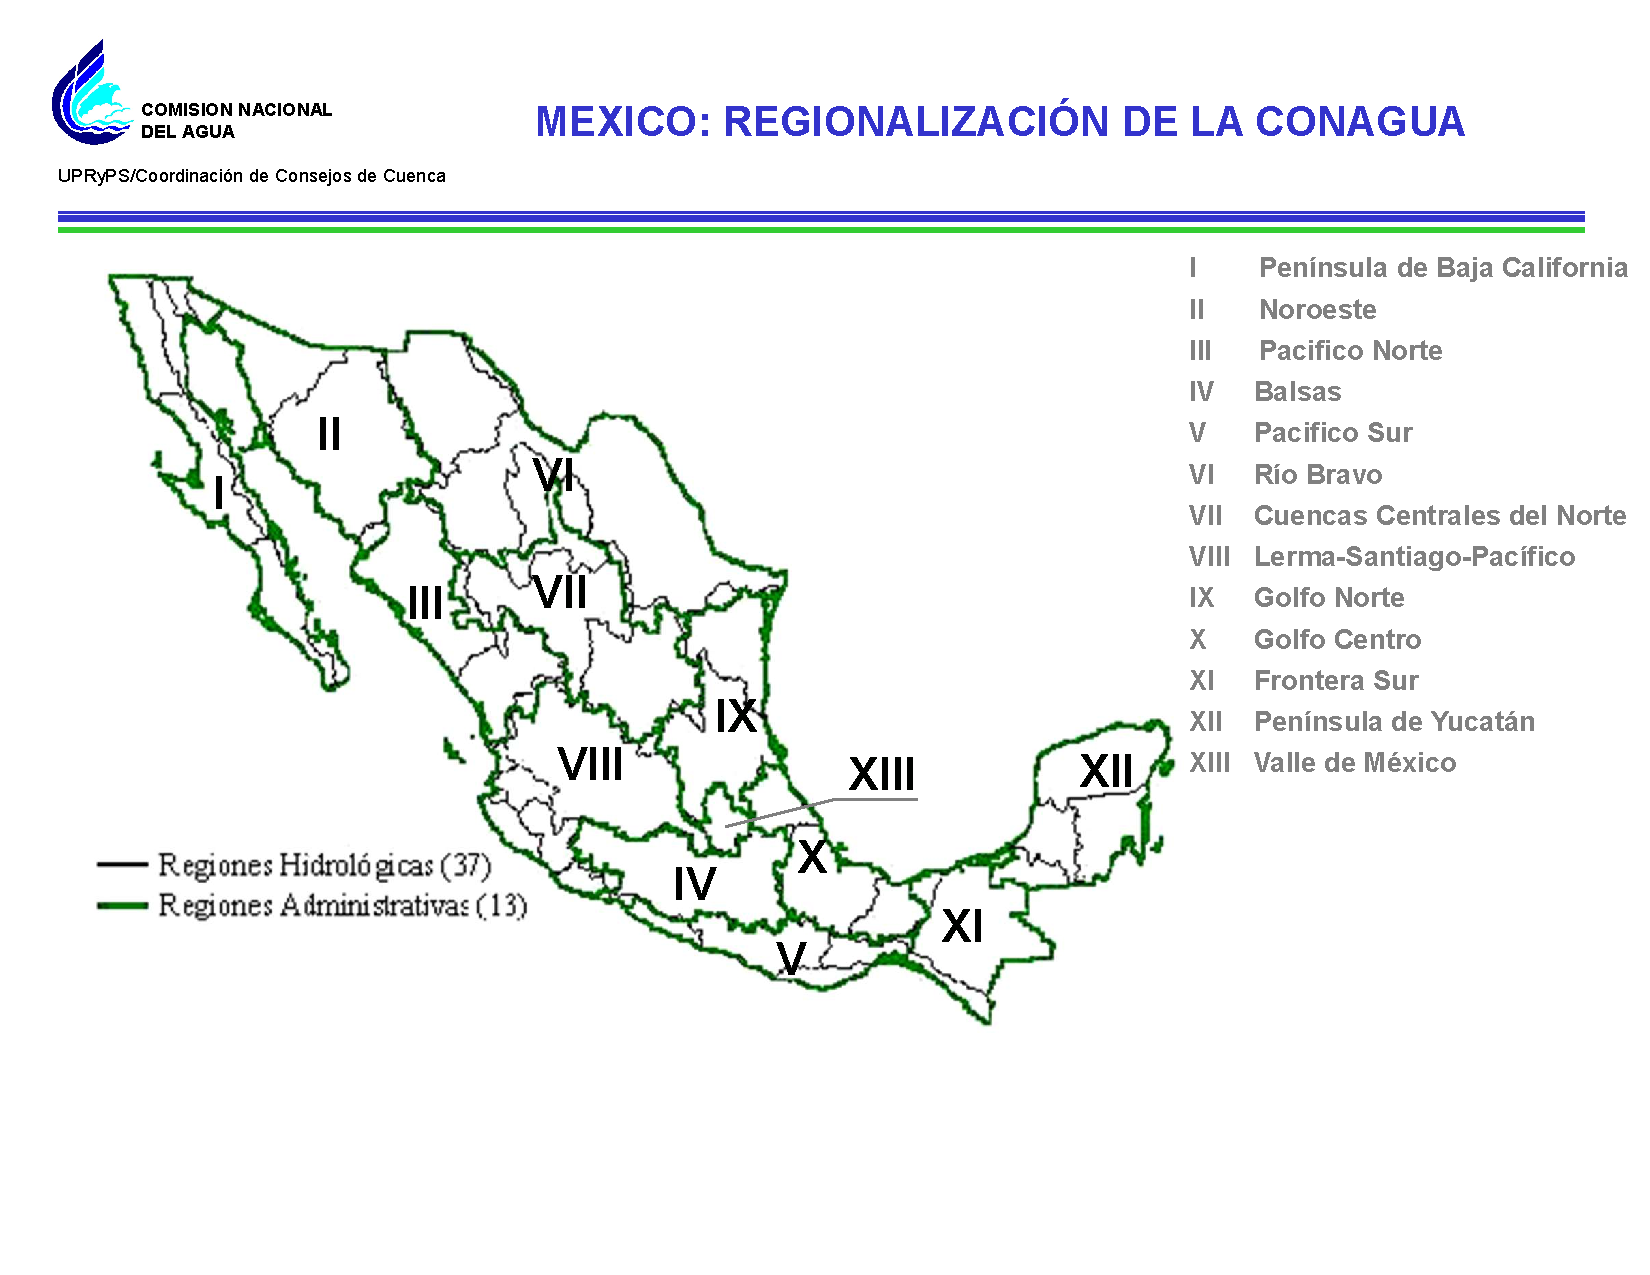
\includegraphics[width=0.5\textwidth]{hs2.pdf}
  \caption{Los limites hidrológicos obedecen criterios geográficos, los limites administrativos obedecen a criterios políticos y de administración.  }
  \label{hs2}
\end{figure}
\begin{figure}[h!]
    \centering
      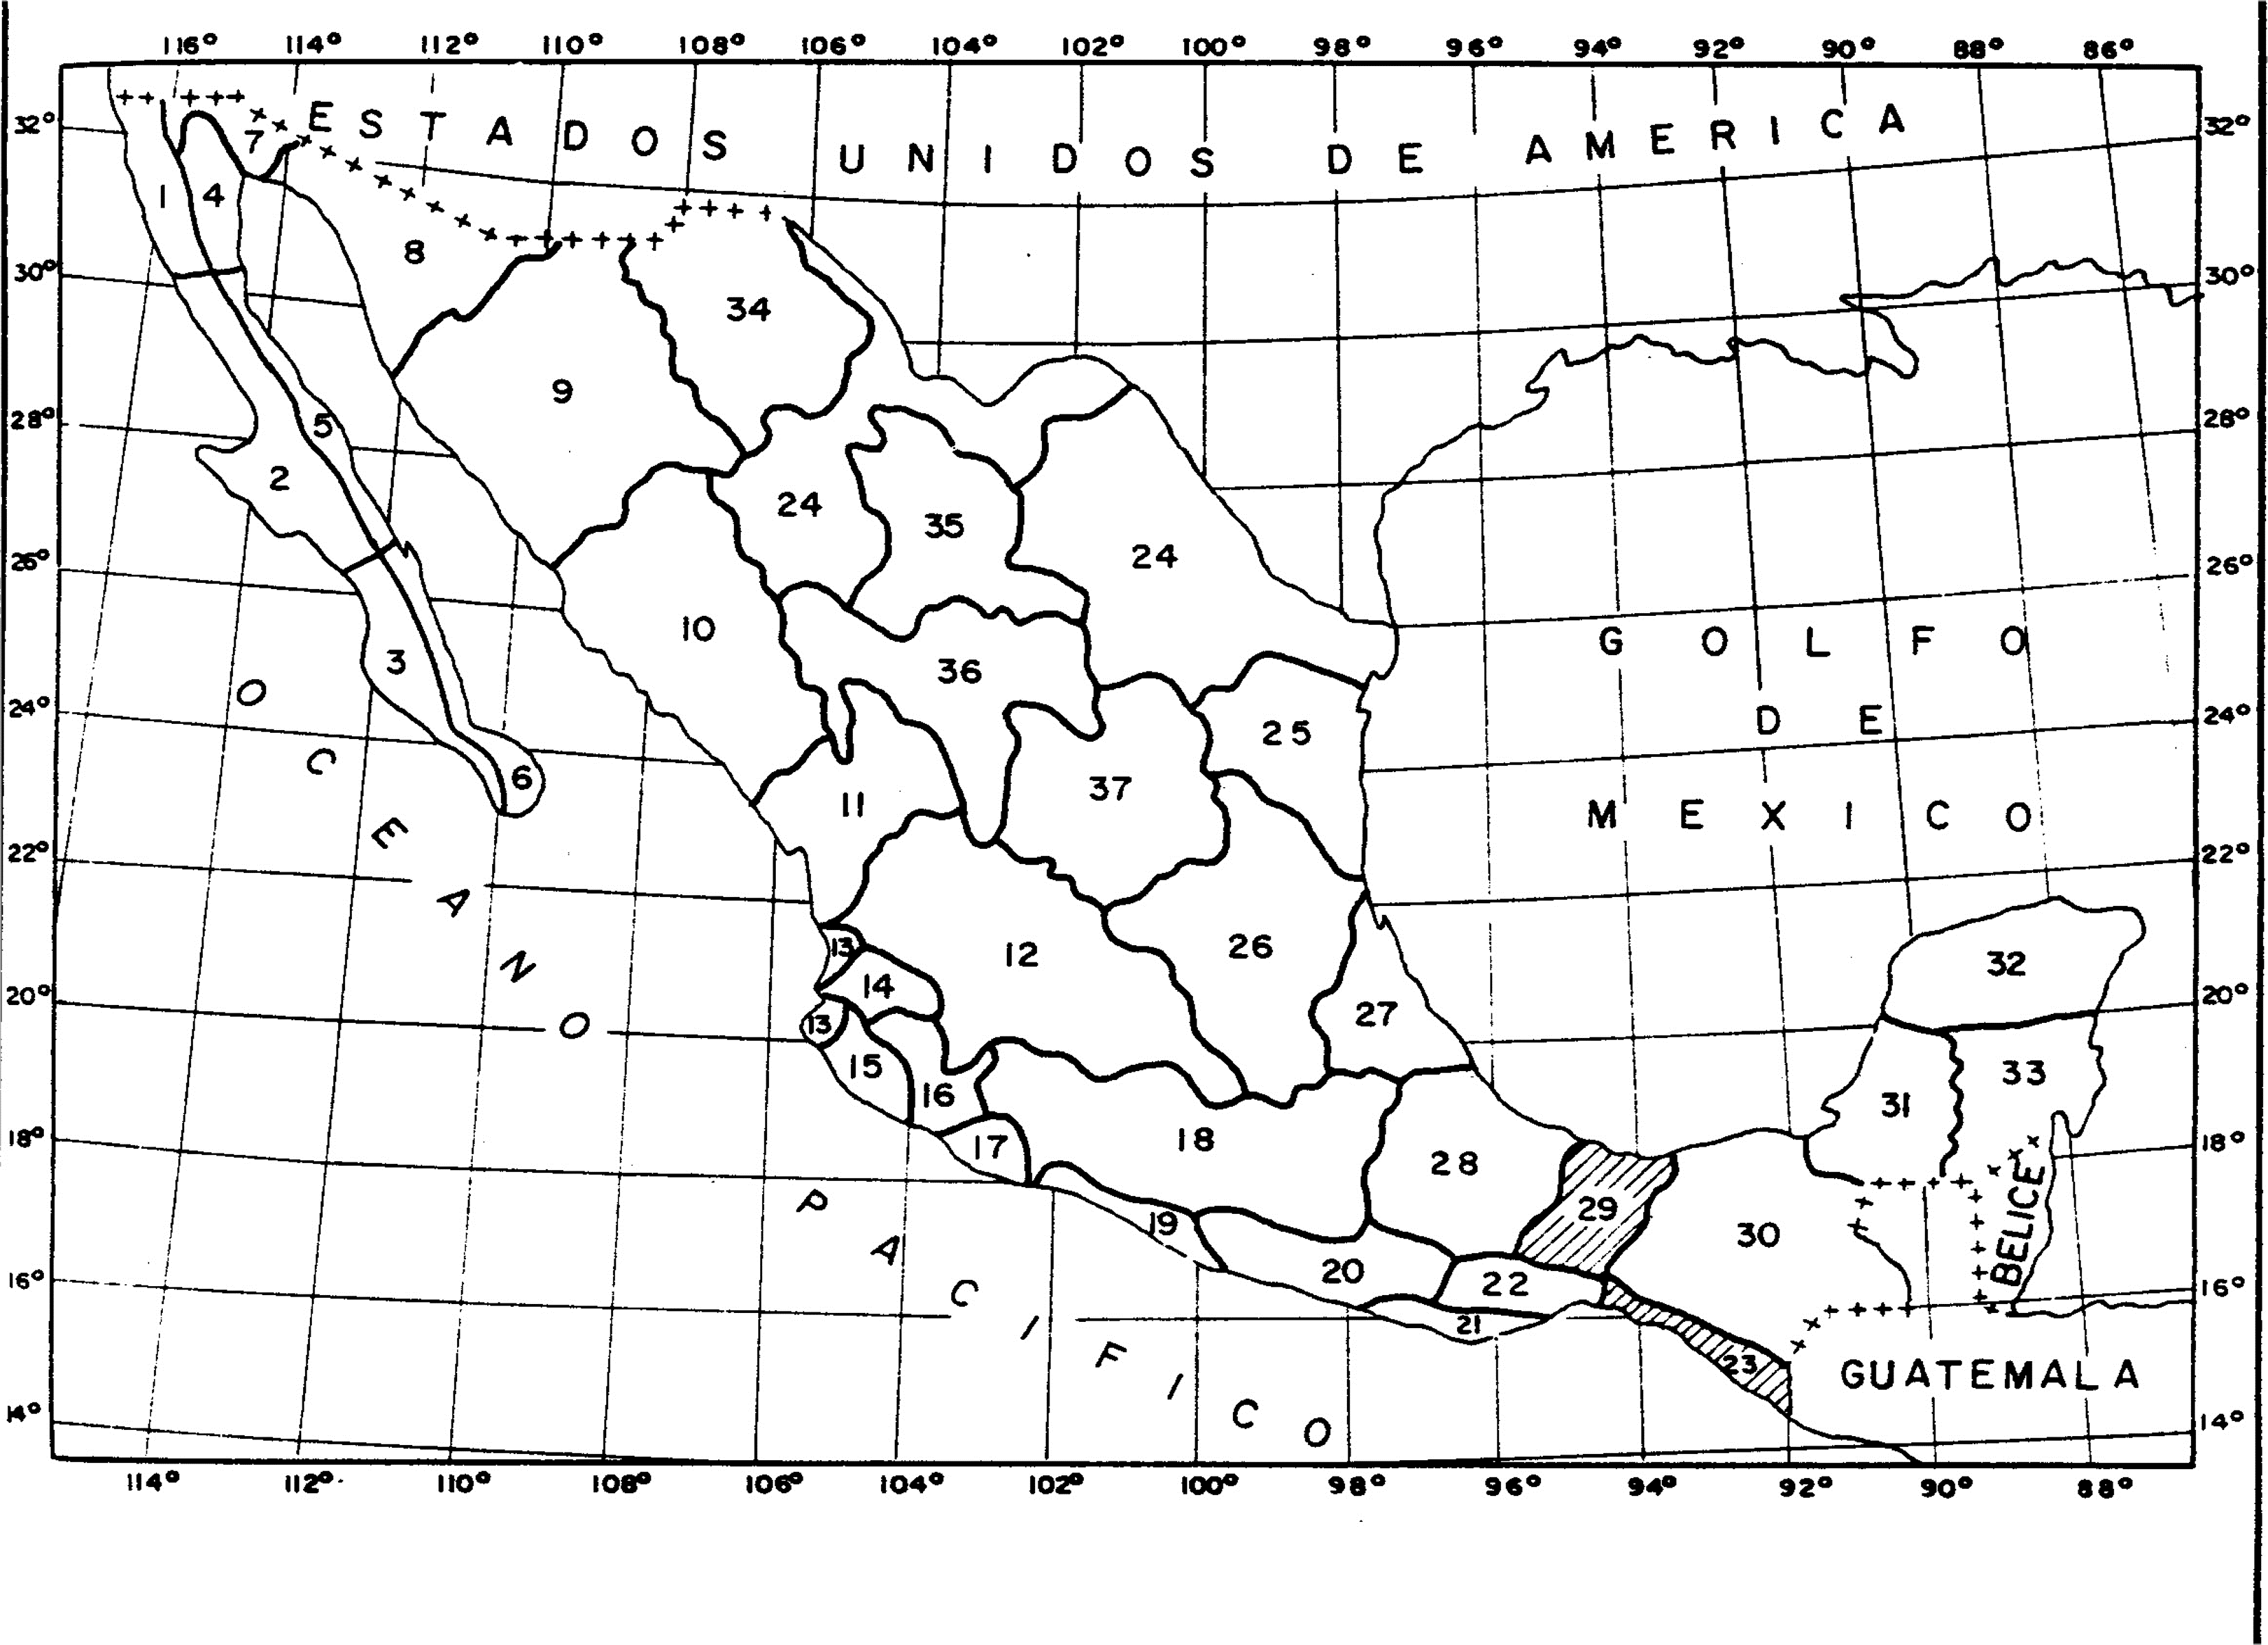
\includegraphics[width=0.5\textwidth]{hs1.png}
      \caption{Regiones hidrológicas de México}
      \label{hs1}
\end{figure}
De la figura \ref{hs1}, puede expresarse que dentro del Estado de México, se concentran las regiones hidrológicas 26 Pánuco 35.4\% (R. Moctezuma, Cuenca lago de Texcoco)
RH-12 Lerma Santiago 23.9\% y la RH-18 Balsas 40.7\% (Sistema Cutzamala) así mismo se tienen 43 presas, las más importantes son:
\begin{itemize}
    \item Presa de \textbf{m3} sobre el R. Ixtapan = 401 millones de $m^3$ (RH Balsas)
    \item Presa \textbf{Villa Victoria} sobre el R. Los Lobos= 218 millones de $m^3$ (RH Balsas)
    \item Huapango sobre el \textbf{R. Huapango} = 130 millones de $m^3$ (RH Pánuco, Municipio. Jilotepec)
    \item Tepetitlán sobre el \textbf{R. Jaltepec} = 92 millones de $m^3$ (RH Lerma, Municipio San Felipe del Progreso)
    \item Presa \textbf{La Angostura en Chiapas} = 19 000 millones de m3
    \item Presa \textbf{MH en Sinaloa} = 3500 millones de m3
\end{itemize}

\begin{definition}[Cuenca]
    es una zona de la superficie terrestre en donde (si fuera impermeable) las gotas de lluvia que caen sobre ella tienden a ser drenadas por el sistema de corrientes hacia un mismo punto de salida.
\end{definition}
La definición anterior se refiere a una cuenca superficial; asociada a cada una de éstas existe también una cuenca de agua subterránea.

Desde el punto de vista de su salida, existen fundamentalmente dos tipos de de cuencas: endorreicas y exorreicas.

Las endorreicas el punto de salida esta dentro de los límites de la cuenca y generalmente es un lago; en las exorreicas su punto de salida esta en los límites de las cuencas y está en otra corriente o mar.

El parteaguas es una línea imaginaria formada por los puntos de mayor nivel topográfico y que separa la cuenca de las cuencas vecinas.

Consultando en el año 2022, las fuentes de información de cuencas y algunos parámetros son:
\begin{itemize}
    \item \textbf{Boletines Hidrológicos} (por región hidrológica)
    \item \textbf{INEGI}: Modelos digitales de elevación, cartas de uso de suelo, cartas edafológicas
    \item \textbf{ERIC III Cd}: Extractor rápido de información meteorológica (editado por el IMTA hasta 2009)
    \item Página Web del \textbf{Servicio Meteorológico Nacional} con datos de climatología diaria y estaciones meteorológicas automatizadas (EMA). Estos datos están actualizados.
    \item \textbf{BANDAS}: Banco Nacional de Datos de Aguas Superficiales en la página web de la CONAGUA
    \item \textbf{Secretaría de Comunicaciones y Transportes} (SCT), con isoyetas de intensidad de la lluvia
    \item \textbf{Imágenes de satélite para usos de suelo} (LANDSAT gratis, SPOT con la Secretaría de Marina Mexicana)
    \item Explorar imágenes de satélite y/o \textbf{radar para lluvia}
\end{itemize}

\subsection{Norma oficial mexicana nom-011-cna-2015 para la conservación del recurso agua que establece las especificaciones y el método para determinar la disponibilidad media anual de las aguas nacionales}
\begin{longtable}[c]{@{}cc@{}}
    \toprule
    Descripción de la Obra Hidráulica &
      Tr \\* \midrule
    \endhead
    %
    \bottomrule
    \endfoot
    %
    \endlastfoot
    %
    \begin{tabular}[c]{@{}c@{}}\textbf{Drenaje pluvial}:\\ Lateral libre en calles de poblados donde se tolera \\ encharcamientos de corta duración\end{tabular} &
      2 \\
    \begin{tabular}[c]{@{}c@{}}Lateral libre en calles de poblados donde no se tolera\\ encharcamiento temporal\end{tabular} &
      5 \\
    De zonas agrícolas &
      5 \\
    \begin{tabular}[c]{@{}c@{}}De zonas urbanas:\\ Poblados pequeños con < de 100,000 habitantes\end{tabular} &
      2 a 5 \\
    Poblados medianos con 100,000 a un millón de habitantes &
      5 a 10 \\
    Poblados grandes con más de un millón de habitantes &
      10 a 25 \\
    Aeropuertos y estaciones de ferrocarril y de autobuses &
      10 \\
    Cuentas y contracuentas en caminos y carreteras &
       \\
    \textbf{Estructuras de Cruce (Puentes y Alcantarillas)} &
       \\
    \begin{tabular}[c]{@{}c@{}}Puentes carreteros en:\\ Caminos locales que comunican poblados pequeños\end{tabular} &
      25 a 50 \\
    Caminos regionales que comunican poblados medianos &
      50 a 100 \\
    Carreteras que comunican poblados grandes (ciudades) &
      500 a 1000 \\
    \begin{tabular}[c]{@{}c@{}}Puentes de ferrocarril en:\\ Vías locales aisladas (desvíos)\end{tabular} &
      50 a 100 \\
    Vías secundarias regionales &
      100 a 500 \\
    Vías primarias del país &
      500 a 1,000 \\
    \begin{tabular}[c]{@{}c@{}}Puentes canales o tuberías en conducción de agua:\\ Para riego en áreas menores de  1,000 Ha\end{tabular} &
      10 a 25 \\
    Para riego en áreas de 1,000 a 10,000 Ha &
      25 a 50 \\
    Para riego en áreas > de 10,000 Ha &
      50 a 100 \\
    De abastecimiento industrial &
      100 a 500 \\
    De abastecimiento de agua potable &
      100 a 500 \\
    \begin{tabular}[c]{@{}c@{}}Puentes para tuberías de petróleo y gas:\\ De abastecimiento secundario local\end{tabular} &
      25 a 50 \\
    De abastecimiento regional| &
      50 a 100 \\
    De abastecimiento primario &
      100 a 500 \\
    \begin{tabular}[c]{@{}c@{}}Alcantarillas para paso de cauces pequeños:\\ En caminos locales que comunican poblados pequeños\end{tabular} &
      10 a 25 \\
    En caminos regionales que comunican poblados medianos &
      25 a 50 \\
    En caminos primarios que comunican poblados grandes &
      50 a 100 \\
    \textbf{Delimitación de zonas federales} &
       \\
    \begin{tabular}[c]{@{}c@{}}Cauces libres en:\\ Zonas semiáridas a húmedas\end{tabular} &
      5 \\
    Zonas áridas con régimen de escurrimiento errático &
      10 o mayor \\
    Zonas de desbordamiento &
      (Nota 1) \\
    \begin{tabular}[c]{@{}c@{}}Cauces con obras de control (además del tramo libre debe\\ tenerse en cuenta el gasto regulado)\end{tabular} &
      (Nota 2) \\
    \textbf{Delimitación de zonas de protección en Obras Hidráulicas} &
      \begin{tabular}[c]{@{}c@{}}A juicio de la \\ CONAGUA*\end{tabular} \\
    \begin{tabular}[c]{@{}c@{}}\textbf{Encauzamiento de Cauces}\\ Corrientes libres en zona:\\ Agrícola de extensión pequeña (< de 1,000 Ha)\end{tabular} &
      10 a 25 \\
    Agrícola de extensión mediana (de 1,000 a 10,000 Ha) &
      25 a 50 \\
    Agrícola de extensión grande (> de 10,000 Ha) &
      50 a 100 \\
    De protección a poblaciones pequeñas &
      50 a 100 \\
    De protección a poblaciones medianas &
      100 a 500 \\
    De protección a poblaciones grandes &
      500 a 1,000 \\
    \begin{tabular}[c]{@{}c@{}}Corrientes controladas:\\ Existe un tramo libre\end{tabular} &
      (Nota 3) \\
    No existe un tramo libre &
      (Nota 4) \\
    \begin{tabular}[c]{@{}c@{}}\textbf{Presas Derivadoras}\\ Para zona de riego pequeña (< de 1,000 Ha)\end{tabular} &
      50 a 100 \\
    Para zona de riego mediana (1,000 a 10,000 Ha) &
      100 a 500 \\
    Para zona de riego grande (> de 10,000 Ha) &
      500 a 1,000 \\
    \begin{tabular}[c]{@{}c@{}}\textbf{Obras de Desvío Temporal}\\ Para presas pequeñas\end{tabular} &
      10 a 25 \\
    Para presas medianas &
      25 a 50 \\
    Para presas grandes &
      50 a 100 \\
    Cauce de alivio en ríos &
      25 a $\geq 50$ \\
    \begin{tabular}[c]{@{}c@{}}\textbf{Presas de almacenamiento}\\ De jales (lodo del procesamiento de minerales en minas)\end{tabular} &
      500 a 1,000 \\
    Para azolve del acarreo del suelo de la cuenca &
      500 a 1,000 \\
    \begin{tabular}[c]{@{}c@{}}Para abastecimiento de agua potable, riego, \\ energía hidroeléctrica, etc\end{tabular} &
      Ver tabla \ref{tabhs3} \\* \bottomrule
    \caption{Periodos de retorno ($Tr$) en años de las crecientes de diseño en diversos tipos de obra hidráulicas}
    \label{tabhs2}\\
\end{longtable}\footnote{Nota 1: Con base en la capacidad del cauce natural cavado; Nota 2: Tr= 5-10 años en ambos o el regulado de diseño de la obra si es superior; Nota 3: Tramo libre igual que inciso 2.1, más gasto regulado para ese periodo de retorno; Nota 4: Igual al gasto de diseño de la obra de controladas}


\subsection{Análisis de frecuencia}
se necesita conocer los volúmenes mensuales de escurrimientos del río que entran a una presa, gastos o caudales de un río, precipitaciones en 24 horas e intensidades de lluvia. Los datos al ser analizados describen eventos aleatorios independientes entre sí, los proceso involucrados son estacionarios a través del tiempo; los parámetros poblacionales pueden ser estimados a partir de una muestra (Discutir población y muestra)
% Se calcula con probabilidad de excedencia, del menor pa arriba
\begin{definition}[Probabilidad de excedencia $(P)$]
    Probabilidad de que un evento de magnitud dada será igualada o excedida dentro de un intervalo de tiempo específico (Usualmente en un año). En distritos de riego, se estiman los volúmenes mensuales de agua que llegan por el río a niveles de probabilidad
\end{definition}
\begin{equation}
    X_T =\bar{x} + k\cdot S_x
\end{equation}
Para la distribución Normal
\begin{equation}
    X_T =\bar{x} + z\cdot S_x
\end{equation}
Éstas ecuaciones nos sirven para calcular los cuantiles, las funciones son:
\subsubsection{Prueba Kolmogorov-Smirnov}
Compara una $F_{teorica}$ se compara con la $F_{observada}$, la mejor distribución es en la cual esa diferencia tiende a cero.
La $F$ teórica es la definición matemática de cada distribución probabilística (Normal, LN)
\begin{equation}
    F_0 = 1 - \frac{m}{n + 1}
\end{equation}
% \subsubsection*{{Error estándar del ajuste}
% \begin{equation}
%     EEA = \sqrt{}
% \end{equation}}
% TODO: EXPLICAR LO DE DISTRIBUCIÖN NORMAL GAMA 3 O PEARSON
El cálculo de un cuantil, significa la ecuación $X_T=\bar{x}+K\cdot S$, 
\begin{notation}
    \begin{itemize}
        \item Donde $T$ es el periodo de retorno ó periodo de recurrencia,
        \item $K$ es el factor de frecuencia, si Pearson III ó Log Pearson III entonces $K=f\left(C_s,T\right)$; eq
        \item Si $x\neq N\left(\bar{x},Sx\right)\implies k=Z$ de las tablas
    \end{itemize}
\end{notation}
\begin{equation}
    F + P_{excedencia} = 1\implies T = \frac{1}{P_{excedencia}}
\end{equation}
cuando $X_T$ y $Vp_{excedencia}$ son desconocidos, entonces se ocupan los momentos y la máxima verosimilitud. Es importante destacar que la distribución probabilística es que en los últimos años, se ha demostrado que el Doble Gumbel es el método más adecuado.
\begin{figure}[h!]
\centering
  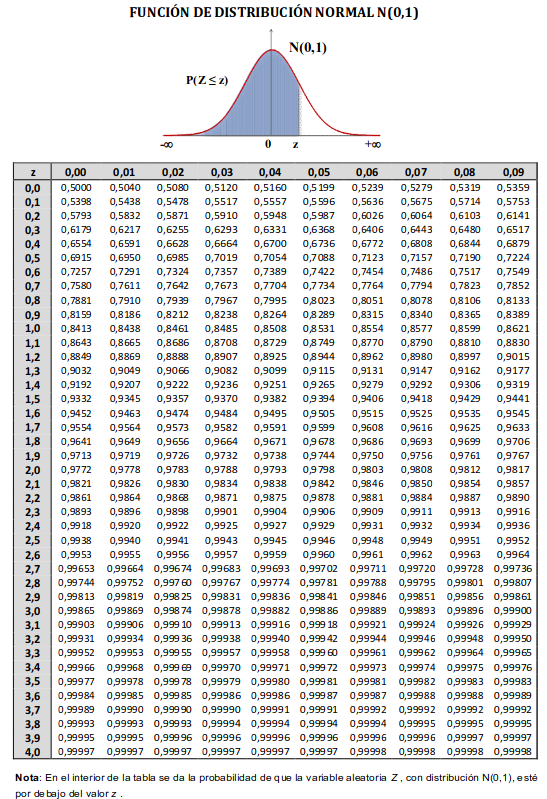
\includegraphics[width=0.5\textwidth]{hs3.png}
  \caption{\textbf{Función de distribución normal (0,1)}, En el interior de la tabla se da la probabilidad de que la variable aleatoria $Z$, con distribución $N(0,1)$ esté por debajo del valor $Z$}
  \label{hs3}
\end{figure}
La prueba de bondad de ajuste que es usada por hidrólogos, son la Kolmogorov-Smirnov, pero también se usa la Xi Cuadrada y la Error Estándar del Ajuste (EEA) donde el valor observada del ajuste, una $f$ empírica, una $F_{tcor}$ y obtenemos para comparar $x_{tcor}$

\begin{example}
    \textbf{Río Siletz}: Calcular el cuartil, ajuste $KS$ y el ajuste $EEA$
\end{example}

\textit{ Sol. }

Recordando la ecuación
\begin{equation*}
    Q_{100} =\bar{Q} + Z\cdot S_Q
\end{equation*}
Entonces calculamos $Z$:
\begin{equation*}
    F = 1 - \frac{1}{T} = 0.99\implies Z
\end{equation*}
De las tablas de datos ($F$), de manera ilustrativa en la tabla:
\begin{table}[h!]
    \centering
    \begin{tabular}{@{}lllll@{}}
    \toprule
    $Z$  & 0.0   & 0.1   & 0.02   & 0.03            \\ \midrule
    -0.1 & \dots & \dots & \dots  & \dots           \\
    2.3  & \dots & \dots & 0.9898 & \textbf{0.9901} \\ \bottomrule
    \end{tabular}
    \caption{Obtención de Z en las tabla }
    \label{tabhs3}
\end{table}
Lo que implica que:
\begin{align*}
    &\bar{Q} =20452&&Q_{100} =20452 +(6089)(2.33)\\
    &S_Q 6089&&Q_{100} = 34639.37
\end{align*}
Entonces haciendo los cálculos de Log Normal 2 par $(\bar{y},S_y)$
Se encuentra $\bar{y}=4.291$ y $S_y=0.129$, así:
\begin{align*}
    Y_{100} = \bar{y} + Z\cdot S_y = 4.291 + (2.33)(0.129) =4.159\\
    Q_{100} = 10^{4.59} = 38904.514
\end{align*}
¿Con qué valor quedarse, con el método Normal ó Log Normal? para eso se hace la prueba de bondad
\section{Precipitación}

Las formas de precipitación son la lluvia, nieve y granizo; Requiere el ascenso de una masa de aire en la atmósfera, de tal manera que esta se enfría y se condensa para formar la lluvia.
Los mecanismos de ascenso de la masa de aire:
\begin{definition}[Convectivo]
    El intenso calor de aire en la superficie, el cual conduce a la expansión y elevación del aire
\end{definition}
\begin{definition}[Elevación por frentes]
    Frentes calientes y frentes frios
\end{definition}
\begin{definition}[Orográfico]
    La masa de aire se eleva al encontrar las montañas para avanzar sobre de ellas.
\end{definition}
\subsection{Condensación}
Para formar nubes se requieren pequeños nucleos de condensación (sal del oceano, polvo de arcillas, productos de combustión industrial,etc.,)

Después por condensación, se van agregando gotas a ese nucleo. La condensación del vapor de agua en nubes cargadas de lluvia ocurre debido al enfriamiento de la humedad del aire a una temperatura por abajo del punto de rocío .

Las gotas se van haciendo más pesadas hasta que son lo suficientemente pesadas para caer en forma de lluvia.

Los tipos de precipitación por la causa de ascenso de la masa de aire húmedo:
\begin{itemize}
    \item Convectivas
    \item Orográficas
    \item Frentes
\end{itemize}
\subsubsection{Medición de la precipitación}
\begin{itemize}
    \item Pluviómetro\footnote{1 mm de lluvia que cae en $1 m^2$, equivale a 1 litro de agua; 1 mm de lluvia qué cae en una hectárea equivale a 10,000 litros}
    \item Pluviógrafo
    \item Estaciones automatizadas
    \item Imágenes de satélite
    \item Radar
\end{itemize}

\subsubsection{Densidad mínima de red pluviométrica}
\begin{itemize}
    \item \textbf{Regiones llanas:} estación para 600 a 900 $km^2$
    \item \textbf{Montañas:} estación para 100 a 250 $km^2$
    \item \textbf{Zonas áridas y polares:} estación para cada 1500 a $10000 km^2$
\end{itemize}
\subsubsection{Clasificación de tormentas}
\begin{itemize}
    \item Lluvia Ligera, en 24 horas llueve de 0.1 a 5 mm
    \item Lluvia Moderada, en 24 horas llueve de 5 a 20 mm
    \item Lluvia Fuerte, en 24 horas llueve de 20 a 70 mm
    \item Lluvia Intensa en 24 horas llueve de 70 a 150 mm
    \item Lluvia Torrencial cuando en 24 horas llueve más de 150 mm\cite{arellano2014estimacion}
\end{itemize}
\begin{table}[h!]
  \centering
  \begin{tabular}{@{}ccccccc@{}}
  \toprule
  \multirow{2}{*}{\begin{tabular}[c]{@{}c@{}}Unidad\\ fisiográfica\end{tabular}} &
    \multicolumn{2}{c}{Precipitación} &
    \multirow{2}{*}{Evaporación} &
    \multirow{2}{*}{Flujo fluvial} &
    \multirow{2}{*}{Sedimentos} &
    \multirow{2}{*}{Calidad del agua} \\
                                                                  & No registradas & Registradas &         &        &         &         \\ \midrule
  Costa                                                           & 900            & 9,000       & 50,000  & 2,750  & 18,300  & 55,000  \\
  Montaña                                                         & 250            & 2,500       & 50,000  & 1,000  & 6,700   & 20,000  \\
  Planicie interior                                               & 575            & 5,750       & 5,000   & 1,875  & 12,500  & 37,500  \\
  \begin{tabular}[c]{@{}c@{}}Montes/\\ ondulaciones\end{tabular}  & 575            & 5,750       & 50,000  & 1,875  & 12,500  & 47,500  \\
  Islas pequeñas                                                  & 25             & 250         & 50,000  & 300    & 2,000   & 6,000   \\
  Áreas urvanas                                                   & -              & 10-20       & -       & -      & -       & -       \\
  \begin{tabular}[c]{@{}c@{}}Polos/\\ Tierras áridas\end{tabular} & 10,000         & 100,000     & 100,000 & 20,000 & 200,000 & 200,000 \\ \bottomrule
  \end{tabular}
  \caption{Valores mínimos recomendados de densidad de estaciones (Superficie, en $km^2$ por estación),}
  \label{tabhs4}
  \end{table}
Algunas bases de datos nacionales de precipitación que se pueden consultar son:
\begin{itemize}
    \item Estaciones meteorológicas locales
    \item Sitio Web del Servicio Meteorológico Nacional (climatología diaria y Estaciones Meteorológicas Automáticas)
    \item CLICOM CICESE
    \item ERIC 
\end{itemize}
\subsubsection{Análisis de una tormenta}
Se debe tomar en cuenta:
\begin{itemize}
    \item El Tirante o lámina precipitada (en México en mm; en USA en pulgadas).
	\item Duración
	\item Distribución en tiempo y espacio
	\item Intensidad (tirante/duración)
	\item Frecuencia (periodos de retorno)
\end{itemize}
\subsubsection{Distribución en tiempo}
\begin{itemize}
	\item Hietogramas de altura (graficas de barras indicando tiempo versus lamina precipitada)
	\item Hietogramas de intensidad (graficas de barras indicando tiempo versus intensidad)
	\item Curva masa de precipitación
\end{itemize}
\subsubsection{Distribución espacial de precipitación}
\begin{itemize}
    \item Método Aritmético
    \item Polígonos de Thiesen
    \item Isoyetas
\end{itemize}
\subsubsection{Características de una tormenta}
\begin{itemize}
    \item Frecuencia (periodos de retorno)
    \item Duración
    \item Distribución en tiempo y espacio
    \item Intensidad (tirante/duración)\footnote{Para caracterizar una tormenta se trabaja con las curvas IDF (intensidad-duración-frecuencia).}
\end{itemize}
\begin{figure}[h!]
\centering
  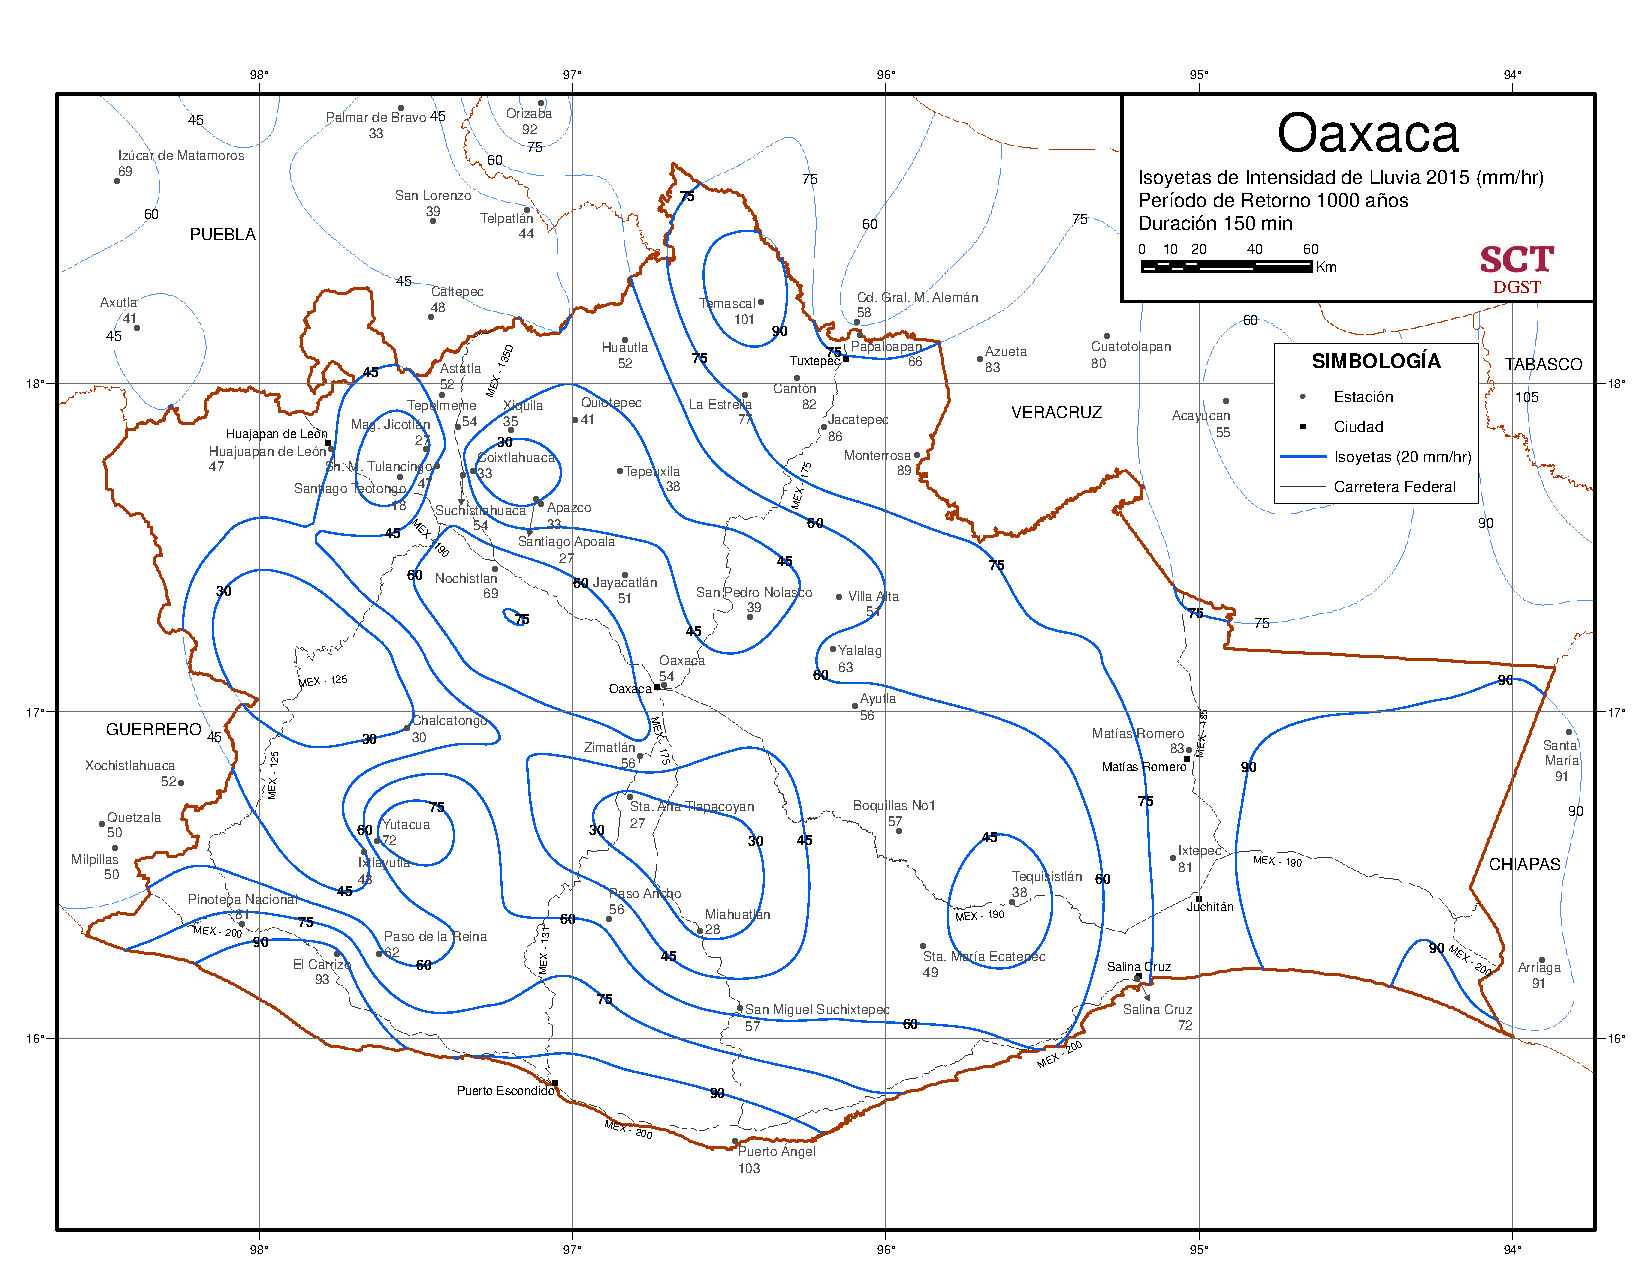
\includegraphics[width=1\textwidth]{hs4.pdf}
  \caption{Secretaría de comunicaciones y transportes: isoyetas de intensidad de la lluvia}
  \label{hs4}
\end{figure}
\subsubsection{Obtención de curvas IDF de la precipitación}
\begin{itemize}
    \item Colección de tirantes históricos extremos anuales para diversas duraciones de lluvias: 5, 10, 20, 30, 40, 50, 60 mins., 2, 3, 4, 5, 10, 15, 24 hs. (cuadro 1)
    \item Sacar intensidades con la información anterior (cuadro 2)
    \item Sacar periodos de retorno de las intensidades históricas del cuadro 2
    \item Regresión lineal múltiple
\end{itemize}
\subsubsection{Relaciones intensidad-duración-frecuencia de la precipitación}
\begin{align}
    &i = \frac{KT^m}{d^n}\\
    &\log{i} =\log{K} + m\cdot\log{T} - n\cdot\log{d}\\
    &Y = a_0 +a_1 \cdot x_1 + a_2 \cdot x_2\\
    &Y = \alpha +\beta_1 \cdot x_1 + \beta_2 \cdot x_2
\end{align}
Regresión lineal múltiple-solución de sistema de ecuaciones normales:
\begin{align}
    &\sum Y =\alpha\cdot \beta_1 \cdot \sum x_1 + \beta_2 \cdot \sum x_2\\
    &\sum\left(x_1 \cdot y\right) = \alpha\cdot\sum x_1 + \beta_1 \cdot \sum \left(x_1\right)^2 + \beta_2\sum x_1 \cdot x_2\\
    &\sum\left(x_2 \cdot y\right) = \alpha\cdot\sum x_2 + \beta_1 \cdot \sum \left(x_1\cdot x_2\right) + \beta_2\sum \left(x_2\right)^2 \\
\end{align}
\begin{notation}
    \begin{itemize}
        \item $Y=\log{i}$
        \item $x_1=\log{T}$
        \item $x_2=\log{d}$
        \item $\alpha=\log{K}$
        \item $\beta_1=m$
        \item $\beta_2=-n$
    \end{itemize}
\end{notation}
% PG 57
\subsection{Datos Faltantes}
No se pueden generar datos de caudales si es que faltan, esto porque la aleatoriedad de la variable es muy alta. Generar datos de precipitación es viable ya que su aleatoriedad es menor al del caudal, aunque el de temperatura es aún menor. Para generar datos faltantes se utiliza el método del U.S. National Weather Service, que es el inverso del cuadrado de la distancia.

Este método funciona al utilizar tres estaciones auxiliares, a las cuales hay que medirles las distancias entre ambas.

\begin{equation}
    W_i = \frac{1}{d_1^2}
\end{equation}
\begin{notation}
Donde:
\begin{itemize}
    \item i=1,2,3
\end{itemize}
\end{notation}
De tal manera que:
\begin{equation}
    P_x=\frac{\sum_{t1}^{n}W_iP_i}{\sum_{t1}^{n}W_i}
\end{equation}
\begin{figure}[h!]
\centering
  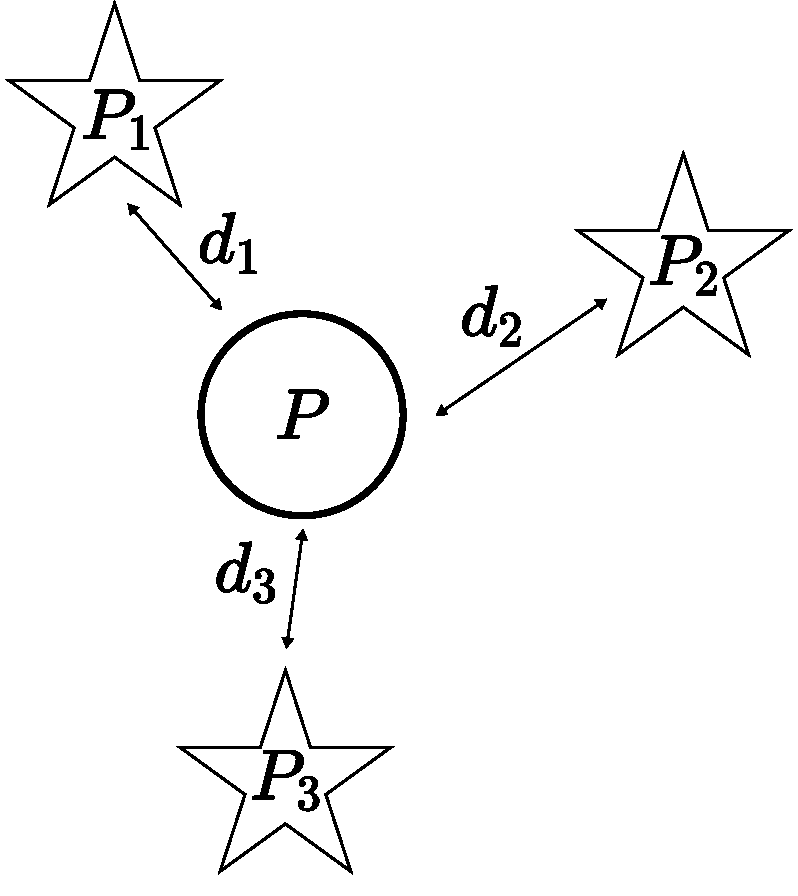
\includegraphics[width=0.5\textwidth]{hs5.pdf}
  \caption{Estimación de datos faltantes de lluvia mediante tres estaciones meteorológica cercanas}
  \label{5}
\end{figure}
\subsection{Métodos para la determinación de las curvas i-d-T}
Existen dos métodos con los que se puede determinar la relación entre las variables intensidad, duración y periodo de retorno (i-d-T). 

El primero llamado ``Intensidad-periodo de retorno'', relaciona estas dos variables para cada duración por separado mediante algunas de las funciones de distribución de probabilidad usadas en hidrología. El segúndo método relaciona simultáneamente las tres variables de una familia de curvas cuya ecuación es la \eqref{eqprec1}:
% \begin{equation}
%     Q = c \cdot i \cdot A
% \end{equation}
% Con la intensidad,duración y frecuencia se pueden generar las isoyetas. En Estados Unidos se usa la ecuación:
\begin{equation}
    i = \frac{k \cdot T^m}{d^n}
    \label{eqprec1}
\end{equation}
donde $k,m,n$ con constantes que se calculan mediante un análisis de correlación lineal múltiple.

Si se toman logaritmos de la ecuación anterior (\eqref{eqprec1}) se obtiene
\begin{equation}
    \log{i} =\log{k} + m \cdot \log{T} - n \cdot \log{d}
\end{equation}
\begin{notation}
    O bien:
\begin{align*}
    &y = a_0 + a_1 \cdot x_1 + a_2 \cdot x_2&&\\
    &a_0 = \log{k}&&x_1 = \log{i}\\
    &a_1 = m&&x_1 = \log{T}\\
    &a_2 =- n&&x_2 = \log{d}  
\end{align*}
\end{notation}
Ésta ecuación es la de una familia de líneas rectas de pendiente $a_2$, ordenada al origen $a_0$ y espaciamiento $a_1$. Si los datos registrados de $i,d,T$ se dibujan en papel logarítmico, usualmente agrupados en torno a líneas rectas. A veces las líneas resultan ligeramente curvas, lo que se puede corregir agregando a las duraciones un valor constante $c$, o bien cuando la pendiente de las líneas varía mucho, dividiendo la línea para cada periodo de retorno en dos rectas. Si los datos se agrupan lo suficiente en torno a líneas rectas, el valor de $c$ puede tomarse como 0.

Al hacer un ajuste de correlación lineal múltiple de una serie de tres tipos de datos, se obtiene un sistema de ecuaciones como el siguiente:
\begin{align*}
    &\sum y = N \cdot a_0 + a_2\sum x_1 +a_2 \cdot \sum x_2\\
    &\sum\left(x_1 \cdot y\right) = a_0 \cdot \sum x_1 + a_1\sum x_1^2 +a_2\sum\left(x_1 \cdot y_2\right)\\
    &\sum\left(x_2 \cdot y\right) = a_0\sum x_2 + a_1\sum\left(x_1 \cdot x_2\right) + a_2\sum x_2^2
\end{align*}
donde $N$ es el número de datos y las incógnitas son $a_0,a_1,a_2$; $x_1,x_2,y$ son respectivamente, los logaritmos del periodo de retorno, la duración (con el valor de $c$ agregado de ser necesario) y la intensidad, obtenidos de un registro de precipitación. Una vez calculados los coeficientes $a_0,a_1,a_2$ es posible valuar los parámetros $k,m,n$ de la ecuación \eqref{eqprec1}.

\subsection{Balance hidrológico}
El modelo más simple está dada en la ecuación \eqref{hp1}
\begin{equation}
    I - Q = \frac{dS}{dt}
\end{equation}
\begin{figure}[h!]
\centering
  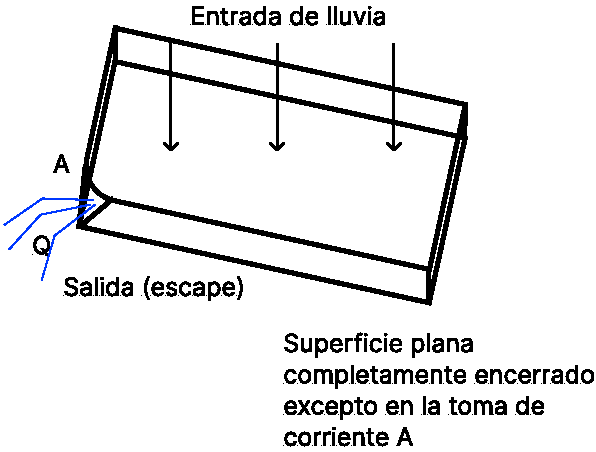
\includegraphics[width=0.5\textwidth]{hs6.pdf}
  \caption{Balance hídrico}
  \label{hs6}
\end{figure}
\begin{equation}
    E - S =\frac{\Delta A}{\Delta t}
\end{equation}
\begin{notation}
    \begin{itemize}
        \item $E$ Entrada de precipitación
        \item $S$ salida
        \item $\Delta A$ cambio de almacenamiento
        \item $\Delta t$incremento del tiempo, semanal, mensual, anual, etc.\cite{viessman1977hydrologic}
    \end{itemize}
\end{notation}
\subsubsection{Recarga potencial es la infiltración}
\begin{equation}
    INFILTRA= P-Q-EVT-INT\quad VEG
\end{equation}
En el enfoque mensual y anual, no todo lo que infiltra recarga
La recarga real se mide con pozos de observación
\begin{figure}[h!]
\centering
  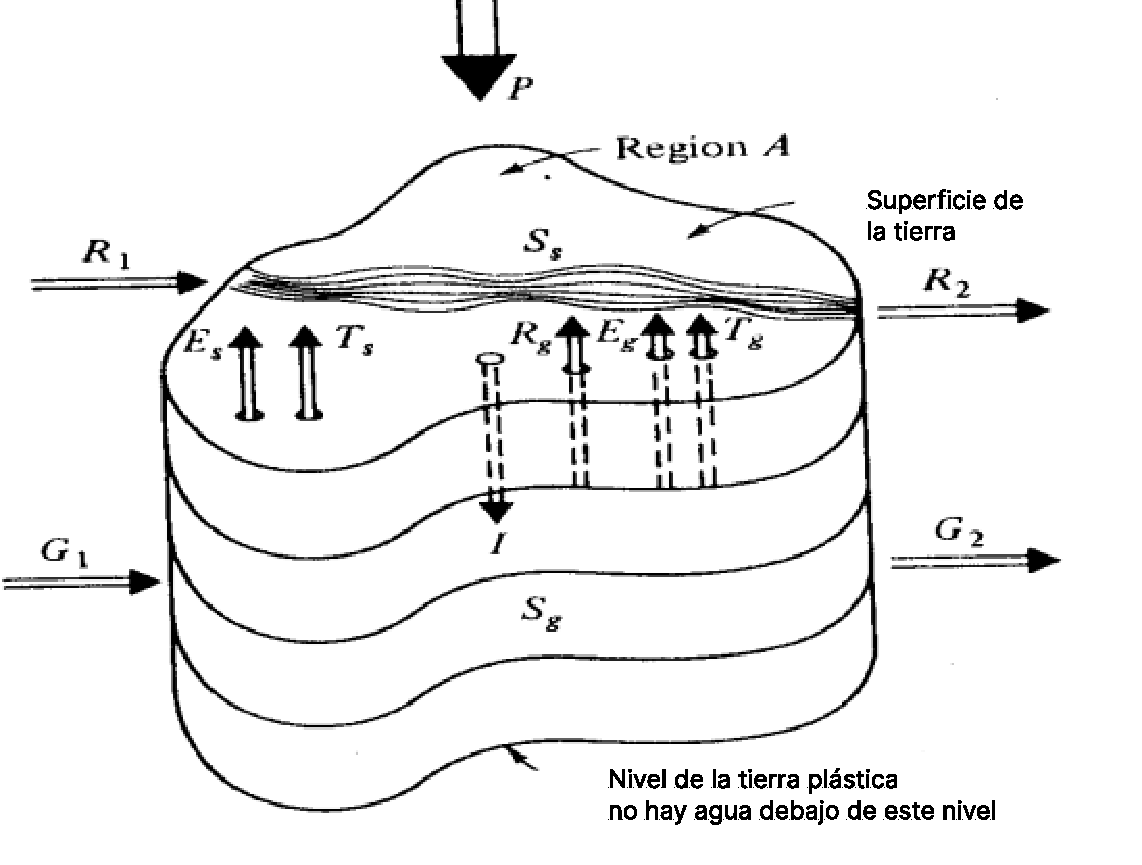
\includegraphics[width=0.5\textwidth]{hs7.pdf}
  \caption{Balance hidrológico para una región en la superficie, subterráneo y global}
  \label{hs7}
\end{figure}
\begin{notation}
    P=precipitación; R= escurrimiento superficial; G= flujo
subterráneo; E = evaporación; T = transpiración. Subíndice g es
para flujo subterráneo; Subíndice s es para flujo superficial.
\end{notation}
% DOS IMAGENEES PENDEINTES EN LA DIAPO SLIDE 1

\subsubsection{Balance hidrológico diario Swat}
\begin{equation}
    SW_t = SW_0 +\sum_{i = 0}^t\left(R_{day} - Q_{surf} - E_a - W_{seep} - Q_{gw}\right)
\end{equation}
\begin{itemize}
    \item $SW_t$ es el contenido final del agua en el suelo para el periodo de tiempo.
    \item $SW_0$ es el contenido inicial de agua del suelo en un día i.
    \item $R_{day}$ es la cantidad de precipitación en un día i.
    \item $Q_{surf}$ es la cantidad de escurrimientos de la superficie en un día i.
    \item $E_a$ es la cantidad de evapotranspiración en un día i.
    \item $W_{seep}$ es la cantidad de agua que percola en el perfil del suelo en día i.
    \item $Q_{gw}$ es la lámina de flujo base en un día i.
    \item Todas las unidades expresadas en mm.
\end{itemize}
Norma oficial mexicana nom-011-cna-2000, ``conservación del recurso agua - que establece las especificaciones y el método para determinar la disponibilidad media anual de las aguas nacionales''. Http://www.Cna.Gob.Mx (normatividad) contenido

\textbf{apéndice normativo ``a''}
métodos para determinar el volumen medio anual de escurrimiento natural

\textbf{apéndice normativo ``b''}
métodos para determinar la recarga total de la unidad
hidrogeológica

\textbf{apéndice informativo ``c''}
ejemplo para determinar mediante el método directo el volumen medio anual de escurrimiento natural

\textbf{apéndice informativo ``d''}
ejemplo para determinar mediante el método indirecto el volumen medio anual de escurrimiento natural

\subsubsection{Escurrimientos por cuenca propia}
Escurrimiento natural: es el volumen medio
anual de agua superficial que se capta por la
red de drenaje natural de la propia cuenca
hidrológica
En NOM-011-CNA se calcula por dos métodos:
\begin{itemize}
    \item Método directo (basado en balance hidrológico superficial)
    \item Método indirecto (con precipitación y coeficientes por tipo y uso de suelo)\footnote{Los cálculos son anuales}
\end{itemize}
\begin{figure}[h!]
\centering
  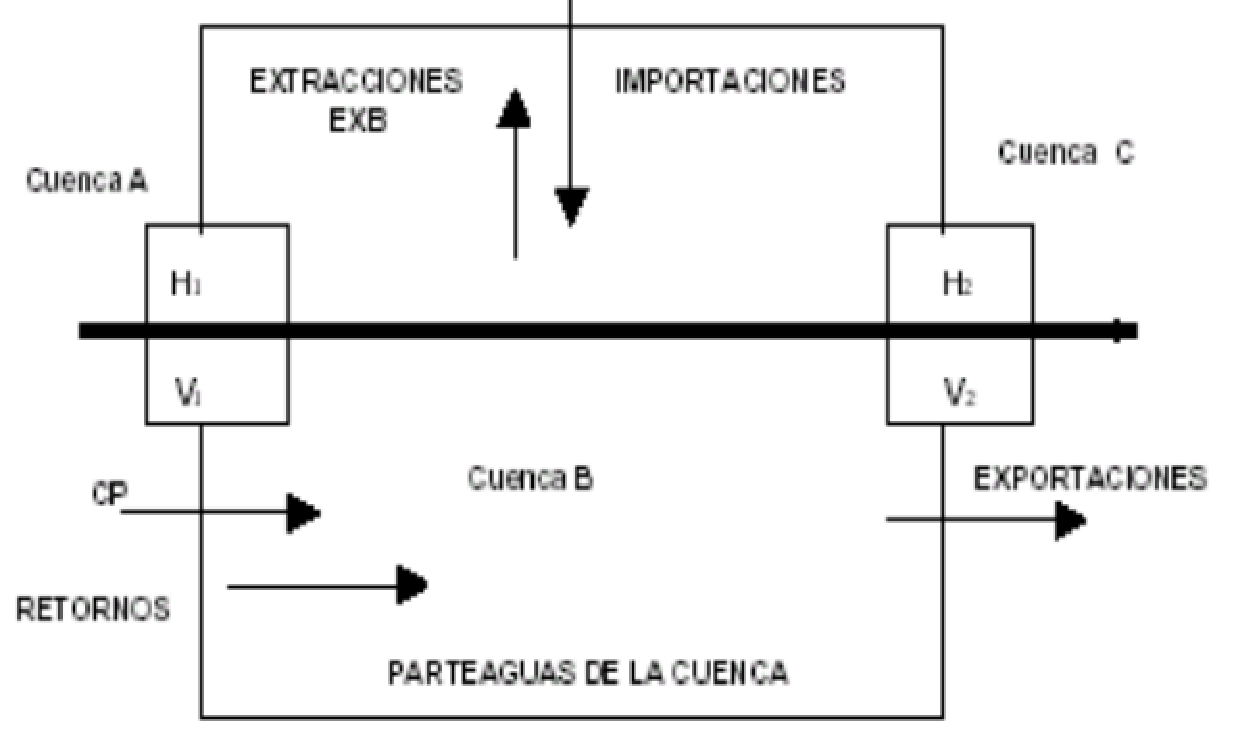
\includegraphics[width=0.5\textwidth]{hs8.pdf}
  \caption{Nom-011-cna. Balance hidrológico superficial para obtener escurrimientos por cuenca propia por el método directo}
  \label{hs8}
\end{figure}
Se determina en el cauce principal en la salida de la cuenca hidrológica, mediante la siguiente expresión, 
\begin{equation}
    Dis = Vol_{med} - Vol_{anual}
\end{equation}
\begin{notation}
    \begin{itemize}
        \item $Dis$: Es la disponibilidad media anual de agua superficial en la cuenca hidrológica
        \item $Vol_{med}$: Volumen medio anual de escurrimiento de la cuenca hacia aguas abajo
        \item $Vol_{anual}$: Volumen anual actual comprometido aguas abajo
    \end{itemize}
\end{notation}
El volumen medio anual de escurrimiento de la cuenca hacia aguas abajo del sitio de interés, se determina al aplicar la siguiente expresión
\begin{equation}
    Vol_{med} = Vol_{cuenca} + Vol_{nat} + Vol_{ret} - Vol_{imp} - Vol_{exp} - Vol_{ext}
\end{equation}
\begin{notation}
    \begin{itemize}
        \item $Vol_{med}$: Volumen medio anual de escurrimiento hacia aguas abajo
        \item $Vol_{cuenca}$: Volumen medio anual de escurrimiento desde la cuenca aguas arriba
        \item $Vol_{nat}$: Volumen medio anual de escurrimiento natural
        \item $Vol_{ret}$: Volumen anual de retornos
        \item $Vol_{imp}$: Volumen anual de importaciones
        \item $Vol_{exp}$: Volumen anual de exportaciones 
        \item $Vol_{ext}$: Volumen anual de extracción de agua superficial
    \end{itemize}
\end{notation}
% Se determina en el cauce principal en la salida de la cuenca hidrológica, mediante la siguiente expresión
% \begin{equation}
%     Disp = Vol_{med} - Vol_{anual}
% \end{equation}
% \begin{notation}
%     \begin{itemize}
%         \item $Disp$ Disponibilidad media anual de agua superficial en la cuenca hidrológica
%         \item $Vol_{med}$ Volumen medio anual de escurrimiento de la cuenca hacia aguas abajo
%         \item $Vol_{anual}$ Volumen anual actual comprometido aguas abajo
%     \end{itemize}
% \end{notation}
% El volumen medio anual de escurrimiento de la cuenca hacia aguas abajo del sitio de interés, se determina al aplicar la siguiente expresión
% \begin{equation}
%     Vol_{med} =
% \end{equation}

Los métodos indirectos, en caso de que en la cuenca en estudio no se cuente con suficiente información de registros hidrométricos ésta sea escasa, para determinar el volumen medio anual de escurrimiento natural se aplica el método directo denominado: precipitación-escurrimiento, el cual es el volumen medio anual de escurrimiento natural, que se determina indirectamente, mediante la expresión siguiente:
\begin{equation}
    Vol_{anual} = Pre_{anual} + A_{cuenca} + C
\end{equation}
\begin{notation}
    \begin{itemize}
        \item $Vol_{anual}$: Volumen anual de escurrimiento natural de la cuenca
        \item $Pre_{anual}$: Precipitación anual de la cuenca
        \item $A_{cuenca}$: Área de la cuenca
        \item $C$: Coeficiente de escurrimiento
    \end{itemize}
\end{notation}
En la precipitación anual en la cuenca, se cuenta con sufciiente información pluviométrica de cuando menos 20 años, la precipitación anual se determina a partir del análisis de los registros de las estaciones ubicadas dentro y vecinas a la cuenca, mediante el método de polígonos de Thiessen o isoyetas



Se pueden estimar como los escurrimientos por cuenca propia de la cuenca. En la NOM-011 es la variable llamada Cp, los cuales pueden ser estimados a partir de datos de aforo o de manera indirecta a falta de aforos

De lo que llueve, una parte escurre y la parte que no escurre, se llama abstracciones.

En las abstracciones se agrupa a la infiltración, la evapotranspiración, y la intercepción vegetal. Cuando se hace el balance hidrológico para una tormenta, la abstracción más importante es la infiltración y la EVT es pequeña. Sin embargo en el balance de un mes o un año, la EVT es significativa.

Los métodos son los siguientes:
\begin{itemize}
    \item Método de Thorntwaite: Aparicio, 2011.
    \item Método de Turc: Campos, 1998. Págs. 7- 47 y 3-7
    \item Método del tanque evaporímetro
    \item Penmann-Monteith, FAO
    \item Penmann-Monteith, Datos estimados
    \item Hargreaves-Samani
    \item Priesley-Taylor
\end{itemize}

Sánchez Galindo y Gamboa Chel, 2011, realizaron un análisis comparativo de tres métodos para estimar la evapotranspiración de referencia en dos condiciones climáticas: Poza Rica, Veracruz (en la costa) y en el Valle de México.

Compararon 3 métodos con el de Penman-Monteith FAO: Penmann-Monteith Datos estimados; Hargreaves-Samani; Priesley-Taylor

Sánchez Galindo y Gamboa Chel, 2011, concluyeron, que a falta de datos para estimar $Eto$ con Penman-Monteith FAO era mejor realizarlo con Priesley-Taylor para ambos climas de la costa y de tierra adentro.

Penman-Monteith FAO: velocidad del viento a 2 m de altura, temperatura del aire a 2 m de altura, presión real de vapor, presión de vapor a saturación, Radiación neta en la superficie del cultivo,

Priestley-Taylor: Temperatura máxima y mínima, temperaturas del bulbo seco y del bulbo húmedo, horas brillo, Radiación solar, altitud

Thornthwaite, 1948: Evapotranspiración potencial es el máximo de evapotranspiración que depende únicamente del clima; no hay restricción de agua en el suelo ($Etp$)

La EVT de referencia, $Eto$, es la evapotranspiración desde una superficie de cultivo hipotético de 0.12 m de altura, la cual se asemeja a una superficie extensa de pasto verde de altura uniforme, en crecimiento y sin limitaciones de agua
\begin{equation}
    ET_o =\frac{0.408\Delta\left(R_n - G\right) +\gamma\frac{900}{T + 273}v_2\left(e_s - e_a\right)}{\Delta + \gamma\left(1 + 0.34v_2\right)}
\end{equation}
\begin{notation}
    \begin{itemize}
        \item $v_2$: Velocidad del viento a 2m de altura (m/s)
        \item $G$ Flujo de calor de suelo ($Mj\cdot m^{-2}$ día$^{-1}$)
        \item $R_n$ Radiación neta en la superficie del cultivo ($Mj\cdot m^{-2}$ día$^{-1}$)
        \item $\gamma$ Constante psicométrica (kPa/C)
        \item $\Delta$ Pendiente de la curva de presión de vapor (kPa/C)
        \item $T$ Temperatura media del aire a 2m de altura ($^{\circ}C$)
        \item $e_a$ Presión real de vapor (kPa)
        \item $e_s$ Presión de vapor de saturación (kPa)
    \end{itemize}
\end{notation}
Evapotranspiración de referencia Hargreaves-Samani
\begin{equation}
        Et_o = 0.0023R_a\left(T + 17.8\right)\left(T_{\max } - T_{\min }\right)^{0.5}
\end{equation}
Evapotranspiración de referencia priesley-taylor
\begin{equation}
    Et_o =\alpha\frac{\Delta}{\Delta +\gamma}\left(R_n - G\right)
\end{equation}
\begin{notation}
    \begin{itemize}
        \item $\alpha$: Constante derivada empíricamente (adim)
        \item $\Delta$: Pendiente de la curva de la presión de vapor saturado a la temperatura promedio del aire (kPa/C)
        \item $\gamma$: Constante psicrométrica (kPa/C)
        \item $R_n$: Radiación neta (mm/día)
        \item $G$: Flujo de calor del suelo (mm/día)
    \end{itemize}
\end{notation}
Radiación neta usada en P-M y Priesley-Taylor
\begin{align}
    &R_n R_{ns} R_{nl}
    &R_{nl} =\sigma\left(\frac{T^4_{\max,k } -T^4_{\min,k }}{2}\right)\left(0.34 -0.14 \sqrt{e_a}\right)\left(1.35\frac{R_s}{R_{so}} - 0.35\right)
    &R_{ns} =\left(1 -\alpha\right)R_s
    &\alpha = 0.23
\end{align}

\subsection{Factores que influyen en el escurrimiento}
\begin{itemize}
    \item Factores meteorológicos
    \item Factores fisiográficos
    \item Factores tipo suelo
    \item Factores uso suelo
    \item Presencia de almacenamientos naturales o artificiales amortiguadores
\end{itemize}
La presencia
\subsubsection{Factores Fisiográficos que influyen en los escurrimientos}
\begin{itemize}
    \item Tamaño y forma del área drenada
    \item Distribución de la red de corrientes
    \item Pendientes de laderas y cauces
    \item Almacenamientos naturales o artificiales que amortiguan avenidas
\end{itemize}
La presencia o ausencia de cubierta vegetal (urbanización) reduce o incrementa las velocidades con que se mueve el agua en la cuenca influenciando el gasto pico. La cubierta vegetal incrementa la cantidad de agua infiltrada en el suelo; La vegetación intercepta lluvia.


\begin{definition}[Aforar]
    determinar a través de mediciones el gasto o caudal (volumen por unidad de tiempo) que pasa por una sección dada
\end{definition}
Se afora generalmente Donde una corriente se une a un cauce principal; Aguas arriba de una población importante. Donde existe la posibilidad de colocar una obra hidráulica importante y/o existe un aprovechamiento de las aguas (agricultura, electricidad, etc.,) Antes de que la corriente desemboque al mar, pero no tan cerca del mar, porqué la marea afecta la medición
\begin{table}[h!]
    \centering
    \begin{tabular}{@{}ccccccc@{}}
    \toprule
    \multirow{2}{*}{Unidad fisiográfica} &
      \multicolumn{2}{c}{Precipitación} &
      \multirow{2}{*}{Evaporación} &
      \multirow{2}{*}{\begin{tabular}[c]{@{}c@{}}Flujo\\ fluvial\end{tabular}} &
      \multirow{2}{*}{Sedimentos} &
      \multirow{2}{*}{\begin{tabular}[c]{@{}c@{}}Calidad\\ de agua\end{tabular}} \\ \cmidrule(lr){2-3}
                                                                   & No registradoras & Registradoras &        &       &        &        \\ \midrule
    Costa                                                          & 900              & 9000          & 50000  & 2750  & 18300  & 55000  \\
    Montaña                                                        & 250              & 2500          & 50000  & 1000  & 6700   & 20000  \\
    Planicie interior                                              & 575              & 5750          & 5000   & 1875  & 12500  & 37500  \\
    \begin{tabular}[c]{@{}c@{}}Montes/\\ ondulaciones\end{tabular} & 575              & 5750          & 50000  & 1875  & 12500  & 47500  \\
    Islas pequeñas                                                 & 25               & 250           & 50000  & 300   & 2000   & 6000   \\
    Áreas urbanas                                                  & -                & 10-20         & -      & -     & -      & -      \\
    Polos/Tierras                                                  & 10000            & 100000        & 100000 & 20000 & 200000 & 200000 \\ \bottomrule
    \end{tabular}
    \caption{Valores mínimos recomendados de densidad de estaciones (Superficie en $km^2$ por estación\textbackslash{}cite\{ibarlucia2017desarrollo\})}
    \label{tabhs5}
\end{table}
\begin{itemize}
    \item Sección de Control (vertedores)
    \item Sección Pendiente (huellas máximas)
    \item Sección área-velocidad (molinete) Curva Elevaciones-Gastos (mantenerla actualizada con datos obtenidos de varios aforos)
\end{itemize}
\subsubsection{Condiciones que debe reunir una estación hidrométrica}
\begin{enumerate}
    \item Accesibilidad: Por ejemplo bajo un puente
    \item Suficiencia: que la medición cubra todo el rango de gastos (mínimo y máximo).
    \item Estabilidad. La sección transversal del río donde se instale la estación debe estar en un tramo recto, lo más estable posible.
    \item Permanencia. La estación debe estar situada de tal manera que nunca sea destruida por una avenida. Una de las características más deseables de un registro es que sea continuo y que esté formado en un mismo sitio.
\end{enumerate}
\subsubsection{Base de datos BANDAS}
Disponibilidad de datos de escurrimiento
2000 estaciones con datos históricos
600 en operación actual (aproximadamente)
\begin{itemize}
    \item Estaciones de nivel
    \item Aforos directos    
\end{itemize}
Curva Elevaciones-Gastos
\begin{equation}
    Q = a\left(H - H_0\right)^b
\end{equation}
\begin{notation}
    \begin{itemize}
        \item $Q$ Gasto en $m^3/s$
        \item $H$ Elevación del nivel del agua, m
        \item $H_0$ Elevación en la cual el gasto es nulo, m
        \item $a,b$ Parámetros de la ecuación.
    \end{itemize}
\end{notation}
Área de un cauce natural:
\begin{equation}
    A = \frac{1}{2}\sum_{i = 1}^n\left[y_1\left(x_{i- 1} - x_{i + 1}\right)\right]
\end{equation}
Actualmente las BANDAS operando son:
\begin{itemize}
    \item DA30019 Serie Anual de Datos
    \item DM30019 Datos mensuales
    \item DD30019 Datos diarios
    \item HD30019 Hidrogramas por evento y subhorarios.
    \item CG30019 Curva Elevaciones-Gastos
\end{itemize}
Determinación de la $Q_{max}$
\begin{itemize}
    \item Fórmulas empíricas
    \item Método de Envolvente máximas por región hidrológica
    \item Método Racional
    \item Análisis de frecuencia de la serie anual de gastos máximos
\end{itemize}
O determinar el hidrograma total a través de la teoría del hidrograma unitario.
\begin{table}[h!]
    \centering
    \begin{tabular}{@{}ccccc@{}}
    \toprule
    No. & Autor     & País    & Fórmula                                                       & \begin{tabular}[c]{@{}c@{}}Limitaciones de las\\ fórmulas\end{tabular} \\ \midrule
    1   & Gete      &         & $Q=(4+15\log{Tr})\sqrt{A}$                                    & Fórmula generalizada en España                                         \\
    2 &
      Morgan &
      Escocia &
      \begin{tabular}[c]{@{}c@{}}$Q_T=52787CA^{0.5}$\\ C=1, Tr=500 años, C=0.454, Tr=40 años\\ C=0.585, Tr=100 años, C)0.215, Tr=5 años\end{tabular} &
       \\
    3 &
      Fuller &
      USA &
      \begin{tabular}[c]{@{}c@{}}$Q_T=Q_m\left(1+0.8\log{Tr}\right)$\\ $Q_m=4\left(1+\frac{266}{400}\right)$\end{tabular} &
       \\
    4 &
      \begin{tabular}[c]{@{}c@{}}Bransby\\ Williams\end{tabular} &
      Inglaterra &
      $Q_m=79.412A^{0.52}$ &
      Áreas mayores de $26km^2$ \\
    5   &           & Francia & $Q_m=150A^{0.5}$                                              & Grandes lluvias $3000km2$                                              \\
    6   &           & Francia & $Q=200A^{0.4}$                                                & $60\leq A\leq 10,000lm^2$                                              \\
    7   & Ryves     & India   & $Q=10106A^{0.5T}$                                             &                                                                        \\
    8   & Valentini & Italia  & $Q=27A^{0.5}$                                                 &                                                                        \\
    9   & Scimemi   & Italia  & $Q_m=\left(\frac{600}{A+10}+1\right)A$                        & Áreas menores de $1,000km^2$                                           \\
    10  & Baratta   & Italia  & $Q_m=\left(\frac{200}{A}+2\right)A$                           & Cuencas monañosas                                                      \\
    11  & Giandotti & Italia  & $Q_m=\left(\frac{332.5}{A+16.2}+5\right)A$                    & Cuencas monañosas                                                      \\
    12 &
      Foreti &
      Italia &
      $Q=\left(2.35\frac{500}{A+125}+0.5\right)A$ &
      \begin{tabular}[c]{@{}c@{}}Lluvias máximas de 200mm\\ en 24 horas\end{tabular} \\
    14  & Myderabad & India   & $Q_w=49.554\left( 0.3861A\right)^{102425\frac{1}{14}\log{A}}$ & Río Tungabhadra                                                        \\
    15  & Creager   & USA     & $Q=39077(0.386A)^{0.2960^{-0.048}}$                           & Avenidas normales                                                      \\ \bottomrule
    \end{tabular}
    \caption{Campos Aranda, 1982. Manual de avenidas máxima}
    \label{tabhs6}
\end{table}
Fórmula empírica de Fuller (U.S.)
\begin{equation}
    Q_{Tr} = Q_m\left(1 +0.8\log{Tr}\right)
\end{equation}
Donde:
\begin{equation}
    Q_m = q\left(1 +\frac{2.66}{A^{0.3}}\right)
\end{equation}
\begin{notation}
    \begin{itemize}
        \item $Q_{Tr}$ Gasto para un periodo de retorno $m^3/s$
        \item $Q_m$ Valor medio de gasto máximo instantáneo, $m^3/s$
        \item $q$ Valor medio de los gastos máximos diarios, $m^3/s$
        \item $A$ Área de la cuenca en $km^2$
        \item $Tr$ Periodo de retorno, años.
    \end{itemize}
\end{notation}
Fórmula empírica de Gete (España)
\begin{equation}
    Q_{Tr} =\left(6 + 16\log{Tr} \right) \sqrt{A}
\end{equation}
\begin{notation}
    \begin{itemize}
        \item $Q_{Tr}$ Gasto para un periodo de retorno, $m^3/s$
        \item $A$ Área de la cuenca en $Km^2$
        \item $T_r$ Periodo de retorno, años
    \end{itemize}
\end{notation}
\subsubsection{Envolventes Actualizadas, 2005}
Se determinaron las envolventes de Creager y Lowry. Adicionalmente, se aplicaron las formulaciones propuestas por Francou-Rodier (1967), Matthai (1969) y Crippen (1982).
Como se ha mencionado, la idea fundamental de todos los métodos de curvas envolventes es relacionar el gasto máximo con un sólo parámetro de la cuenca; el área. A continuación se presentan las formulaciones aplicadas

Envolvente de Creager: Creager et al (1945) introdujeron la envolvente de más uso en el mundo con el fin de estimar la magnitud de eventos extraordinarios en los Estados Unidos. La ecuación propuesta es:
\begin{equation}
    q = 1.303C_c\left(0.386A\right)^{0.935A^{ -0.048}}A^{ -1}
\end{equation}
Donde $q$ es el gasto específico o gasto por unidad de área en $m^{3}/s/km^2$, $A$ es el área de la cuenca en $km^2$ y envolvente de Lowry es muy usada en Latinoamérica. La expresión par el cálculo del gasto específico está dada por:
\begin{equation}
    a =\frac{C_L}{\left(A + 259\right)}^{0.85}
\end{equation}
Donde $C_L$ es un parámetro empírico y A es el área de la cuenca en $km^2$.

En 1978, la SARH publicó los valores del coeficiente de Lowry para cada una de las 37 regiones hidrológicas previamente definidas. Para el cálculo de los coeficientes se utilizaron datos observados de gastos máximos hasta 1975. Con esos datos, la envolvente nacional estaba dada por $C_L=5270$, valor estimado para la región Costa de Jalisco (SARAH, 1978).

\section{Hidrograma}
Un hidrograma es una gráfica continua tiempo contra gasto
(volumen / unidad de tiempo) producido por una lluvia de
cualquier magnitud para una duración específica. Un
hidrograma puede ser el resultado de un proceso de aforos
en un río.
Sus componentes consisten en \begin{itemize}
  \item  Flujo superficial ó Escurrimiento directo (pudiendo incluir interflujo)
  \item Flujo Base o Flujo subterráneo somero
\end{itemize}
\subsection{Hidrograma Unitario (Sherman, 1932; Horton, 1933)}
El hidrograma que resulta de 1-mm de lluvia exceso (o 1 pulgada o 1
cm) distribuido uniformemente en espacio sobre un área para una
duración dada.

Los puntos clave:
\begin{itemize}
  \item 1-mm de lluvia EXCESO
  \item La lluvia exceso está distribuída uniformemente en espacio sobre un área
  \item La lluvia exceso tiene una duración asociada
\end{itemize}

\subsubsection{Volúmenes escurridos}
\begin{itemize}
  \item Anuales, mensuales: NOM011 CONAGUA
  \item Diarios: Número de curva de escurrimiento del SCS con la precipitación en 24 horas registrada por pluviómetro
  \item Subhorarios: Número de curva de escurrimiento del SCS con la precipitación expresada como hietograma de lámina (pluviografo o EMA)
\end{itemize}
\subsubsection{Método racional}
\begin{equation}
  Q =k \cdot CIA
\end{equation}
No confundir con la NOM011 CONAGUA que determina volúmenes en miles $m^3$:
\begin{equation}
  V_{anual}= C \cdot P_{anual}A\quad NOM011
\end{equation}
\subsubsection{Métodos para determinar el Hidrograma Unitario}
A partir de medición: hietograma e hidrograma
\begin{itemize}
    \item Tradicional
    \item Instantaneo o matricial
\end{itemize}
Sintéticos
\begin{itemize}
    \item Hidrograma unitario triangular (HUT) del SCS
    \item Hidrograma unitario curvilineo o adimensional del SCS
    \item Snyder
    \item Clark    
\end{itemize}
\subsubsection{Método Tradicional}
\begin{enumerate}
    \item Separar flujo base de flujo directo
    \item Cálculo del volumen de escurrimiento directo. Medir el volumen total bajo el hidrograma
    \item Cálculo de la altura de precipitación efectiva : dividir Vol. Esc. Directo entre area de la cuenca y obtenerlo en mm o cm o pulgadas
    \item Derivar las ordenadas del hidrograma unitario dividiendo las ordenadas del hidrograma total entre la altura precipitación efectiva del punto 3
    \item Determinar duración efectiva separando lluvia efectiva e infiltración y viendo la duración de la lluvia efectiva (en este momento hacerlo con el indice de infiltración media)
\end{enumerate}
\begin{example}
    Determinar H.U. para una cuenca de 888 $Km^2$ Hietograma de altura de precipitacion, con el método tradicional
\textit{ Sol. }
\begin{table}[h!]
    \centering
    \begin{tabular}{@{}cc@{}}
    \toprule
    Tiempo (horas) & Precipitación Hp (mm) \\ \midrule
    0-2            & 7.0                   \\
    2-4            & 9.0                   \\
    4-6            & 4.0                   \\
    6-8            & 1.0                   \\
    8-10           & 2.0                   \\ \bottomrule
    \end{tabular}
    \caption{Hoja de cálculo}
    \label{tabhs7}
\end{table}
\end{example}

\begin{example}
    Hidrograma de escurrimiento medido a la salida de la cuenca con el método tradicional:
    \begin{table}[h!]
        \centering
        \begin{tabular}{@{}cc@{}}
        \toprule
        \begin{tabular}[c]{@{}c@{}}Tiempo\\ (horas)\end{tabular} & \begin{tabular}[c]{@{}c@{}}Gasto\\ $Q (m^3/s)$\end{tabular} \\ \midrule
        0  & 40.0  \\
        2  & 80.0  \\
        4  & 220.0 \\
        6  & 300.0 \\
        8  & 200.0 \\
        10 & 120.0 \\
        12 & 60.0  \\
        14 & 40.0  \\ \bottomrule
        \end{tabular}
        \caption{Hoja de cálculo con el método tradicional}
        \label{tabhs9}
        \end{table}
\end{example}

\subsubsection{Hidrogramas Unitarios Sintéticos}
\begin{itemize}
    \item Chow
    \item SCS (triangular y curvilíneo)
    \item Snyder
    \item Clark
\end{itemize}
Hay para cuencas no aforadas y se usan las características generales de las cuencas fáciles de obtener (área, pendientes,tiempo de concentración), por lo que se utilizan formulas empíricas para obtener todos los parámetros del hidrograma unitario
\subsubsection{H.U. SCS parámetros}
\begin{itemize}
    \item Tiempo de concentración $t_c$
    \item Tiempo de retraso ó lag-time $t_r$
    \item Duración efectiva de la lluvia $\Delta T$
    \item Tiempo al pico $t_p$
    \item TIempo base $t_b$
    \item Caudal pico $q_p$
\end{itemize}
\subsubsection{HUT SCS gasto pico}
A Partir de la geometría de la figura y con la debida conversión de unidades:
\begin{equation}
    q_p = \frac{0.208 A_c}{t_p}
\end{equation}
\begin{notation}
    \begin{itemize}
        \item $A$ Área de la cuenca en $km^2$
        \item $t_p$ tiempo al pico en horas
        \item $q_p$ gasto pico unitario en $m^3/s/mm$
    \end{itemize}
\end{notation}
De acuerdoa Mockus(analisis de hidrogramas):
\begin{equation}
    t_b = 2.67 \cdot t_p
\end{equation}
De acuerdoa la figura :
\begin{equation}
    t_p = \frac{d_e}{2} + t_r
\end{equation}
De acuerdoa Mockus\footnote{Depende del tiempo de concentración}:
\begin{align}
    &t_r = 0.6 \cdot t_c\\
    &d_e = 0.1333 \cdot t_c
\end{align}
Una mejora al planteamiento del HUT de libro de Aparicio, 2001 para poder usarse para fines prácticos

Cuando se tiene un hietograma de lluvia, digamos, cada 10 minutos, llamémosle $\Delta t=10$ minutos

Por lo tanto querremos un HU cuya duración efectiva sea igual a $\Delta t$ (de= $\Delta t\leq 0.29 t_r$), por lo que quedarían así estas dos ecuaciones:
\begin{align*}
    &q_p = \frac{0.208 A_c}{t_p}\\
    &t_p = \frac{\Delta t}{2} + t_r
\end{align*}
De esta forma nos evitamos estar cambiándole la duración efectiva al HU. Simplemente lo generamos para la duración efectiva que queremos (USACE, 2000)
\subsubsection{Tiempo de concentración}
Con la ecuación de Kirpich o con la formula empírica de tiempo de concentración delSCS (horas):
\begin{equation}
    t_c =\frac{0.00227 \cdot L^{0.8}\left(\frac{100}{CN} - 9\right)^{0.7}}{Y^{0.5}}
\end{equation}
\begin{notation}
    \begin{itemize}
        \item L Longitud del cauce ppal.en m (longest flow path)
        \item Y pendientepromedio de cuenca en \%;CN numero curva\footnote{Recordar que tr = 0.6 tc}
    \end{itemize}
\end{notation}
\subsubsection{H.U. Sintético Curvilíneo del SCS}
Se requiere $q_p$ y $t_p$:
\begin{align}
    t_p = \frac{2}{3}t_c\\
    q_p = \frac{0.208 \cdot A_c}{t_p}\\
    t_c =\frac{0.00227 \cdot L^{0.8}\left(\frac{1000}{CN} 9\right)^{0.7}}{Y^{0.5}}
\end{align}
\subsubsection{H.U. Sintético Curvilíneo del SCS}
\begin{itemize}
    \item Se debe tener calculado el tp y qp
    \item Para encontrar abscisas del hidrograma se multiplica el “time ratio” por el tiempo al pico (tp )
    \item Para encontrar las ordenadas del hidrograma se multiplica el “Discharge ratio” por el gasto pico (qp)
\end{itemize}

\subsection{Calculo del Caudal Máximo}
Para obtener éste caudal de para diseño, se usan los siguientes métodos:
\begin{itemize}
    \item Análisis de frecuencia (ideal)
    \item Método racional
    \item Las envolventes máximas por región hidrológica
    \item Hidrograma unitario: Cerca de cuatro sub-métodos faciales de usar.
\end{itemize}
\section{Tránsito de avenidas}
\begin{definition}[Avenida o creciente]
    Es un cambio rápido del gasto o caudal que cruza un río o una presa. Dicho cambio es casi siempre debido a una tormenta. Originando con ello un hidrograma donde claramente esta definido una rama ascendente, un pico y una rama descendente
\end{definition}
% \begin{center}
%     \smartdiagramset{border color=none,
%     uniform color list=teal!60 for 4 items,
%     arrow style=[-stealth’,
%     module x sep=3.75,
%     back arrow distance=0.75,
%     }
%     \smartdiagram[flow diagram:horizontal]{Lámina precipitada,Lámina escurrida,Hidrograma,Hidrograma transitado en cauces,Hidrograma transitado en presas, Hidrograma a la salida}
% \end{center}
\begin{figure}[h!]
\centering
  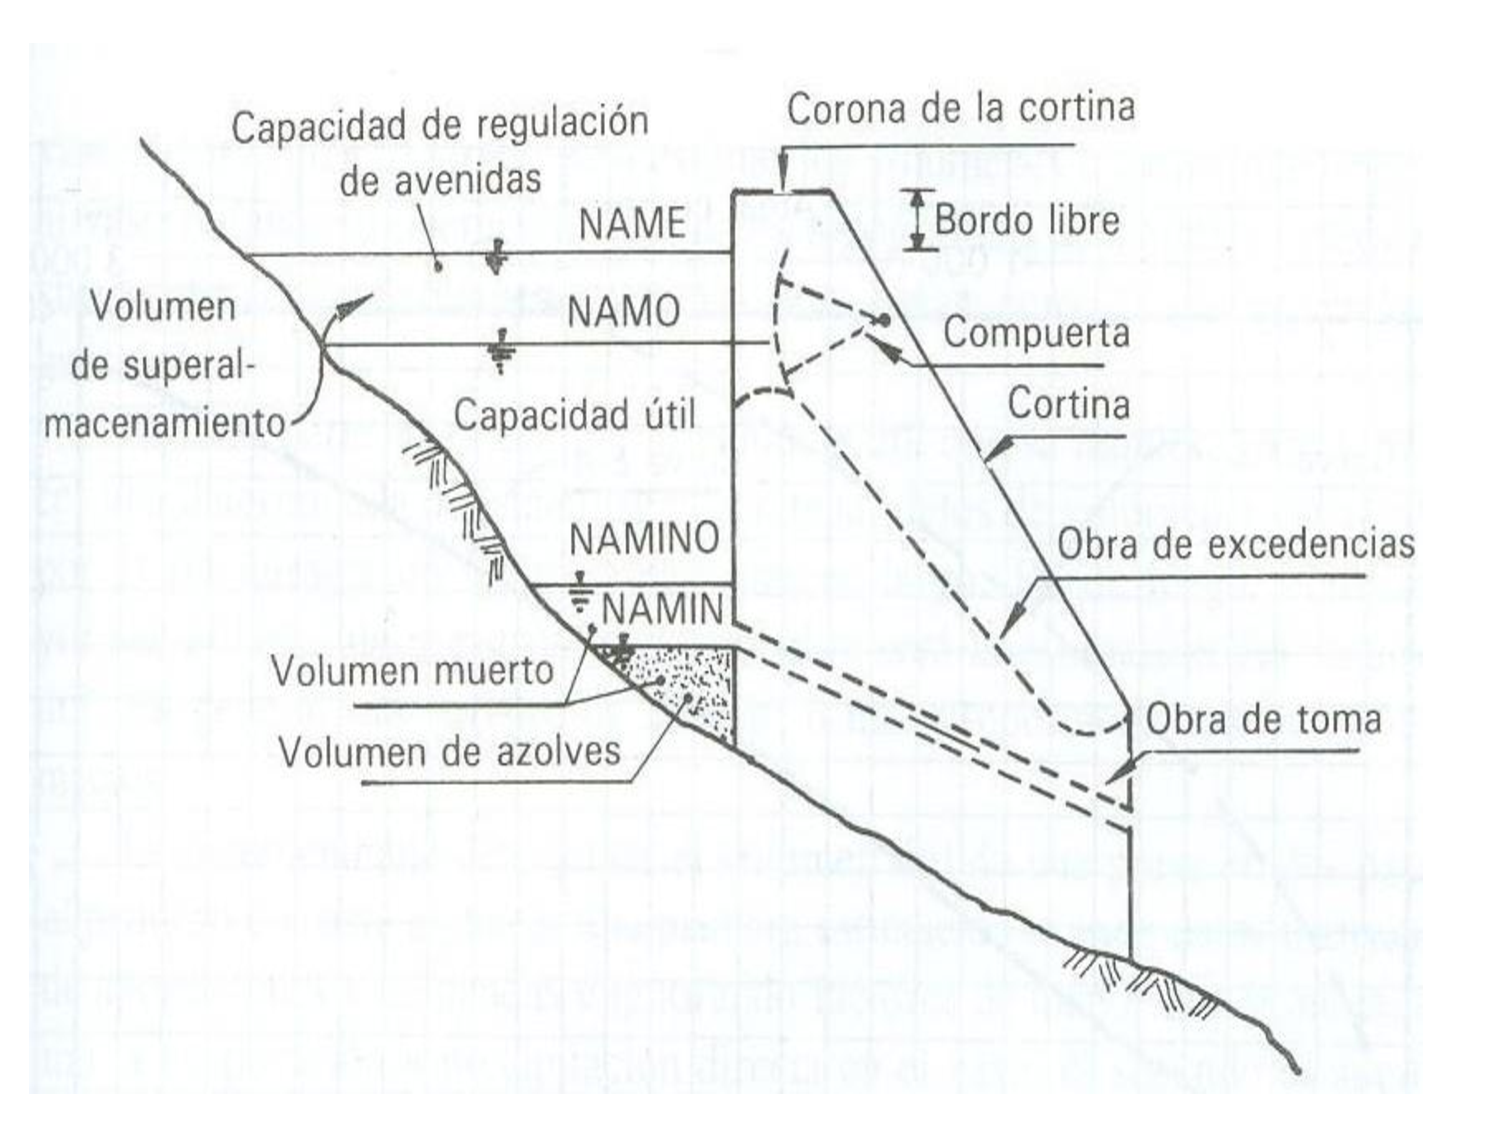
\includegraphics[width=0.5\textwidth]{hs9.pdf}
  \caption{Partes de una cortina}
  \label{hs9}
\end{figure}
\begin{definition}[Transitar la avenida]
    Significa simular que dicha avenida cruza o transita la presa y calcular el efecto amortiguador que tiene el almacenamiento sobre el pico y tiempo de ocurrencia del pico del hidrograma. Es decir, hay un hidrograma de entrada y uno de salida que esta “achatado” y “barrido
\end{definition}
\begin{equation}
    I - 0 =\frac{dV}{dt}
\end{equation}
O bien, en diferencias finitas:
\begin{equation}
    \frac{I_i + I_{j + 1}}{2} -\frac{O_i + O_{i + 1}}{2} =\frac{V_{i+ 1} - V_i}{\Delta t}\mid \Delta t\leq 0.1t_p
\end{equation}
Ecuación para tránsito de avenidas basada en continuidad en el vaso
\begin{equation}
    \label{eqhs1}
    I_i + I_{i + 1} +\left(\frac{2V_i}{\Delta t} - O_i\right) =\frac{2V_{i + 1}}{\Delta t} + O_{i + 1}
\end{equation}
\begin{notation}
    \begin{itemize}
        \item $I=$ Gasto de hidrograma de entrada
        \item $V=$ Volumen almacenado en la presa
        \item $O=$ Gasto de hidrograma de salida
        \item $i=$ Ordenada para el i-ésimo tiempo t
        \item $\Delta t=$ Incremento de tiempo usado para el funcionamiento del vaso
    \end{itemize}
\end{notation}
\begin{example}
    Transitar la avenida mostrada por un vaso cuya curva de elevaciones y volúmenes tiene la ecuación:
    \begin{equation*}
        V = 10E^{ - 1.18}
    \end{equation*}
    donde $E=$eñevación en m  $V=$ volumen en miles de $m^3$. La elevación del NAMO es la 50.4m, el vertedor es de cresta libre con longitud de 15m y coeficiente de descarga de 2. La salida por la obra de toma es constante e igual a $20m^3/s$
\end{example}
\textit{ Sol. }

\begin{align*}
    0 = CL\left(E - E_Q\right)ñ\frac{3}{2} + O_T\\
    = 2 \cdot 15\left(E - 50.4\right)^{\frac{3}{2}} + 20 = 30\left(E - 50.4\right)^{\frac{3}{2}} + 20\\
    \text{si }E > 50.4m\quad \text{si }E < 50.4m,\, O = O_T = \frac{20m^3}{s} \mid \Delta t = 0.1hr = 360seg
\end{align*}
\begin{table}[h!]
    \centering
    \begin{tabular}{@{}cccc@{}}
    \toprule
    \begin{tabular}[c]{@{}c@{}}E\\ m\end{tabular} &
      \begin{tabular}[c]{@{}c@{}}V\\ $10^3m^3$\end{tabular} &
      \begin{tabular}[c]{@{}c@{}}O\\ $m^3/s$\end{tabular} &
      \begin{tabular}[c]{@{}c@{}}$\frac{2V}{\Delta t}+O$\\ $m^3/s$\end{tabular} \\ \midrule
    50.4 & 1020.6 & 20    & 5690   \\
    51   & 1035   & 33.9  & 5783.8 \\
    52   & 1059   & 80.7  & 5963.9 \\
    53   & 1083   & 145.8 & 6162.7 \\
    54   & 1107.2 & 224.9 & 6376   \\ \bottomrule
    \end{tabular}
    \caption{Se grafica col. 4 vs. col. 3}
    \label{tabhs10}
\end{table}
\begin{figure}[h!]
\centering
  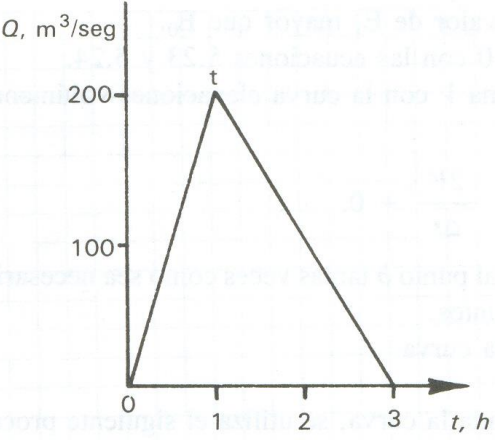
\includegraphics[width=0.5\textwidth]{hs10.png}
  \caption{Hidrograma de entradas}
  \label{hs10}
\end{figure}
Usando la ecuación \eqref{eqhs1}, podemos obtener la siguiente tabla:

¿Cómo calcular las columnas 8 y 9?

La columna 8 se despeja del valor de la columna 5
\begin{equation}
    \left(\frac{2V_i}{\Delta t} - O_i\right) =\text{Valor de la columna 5}
\end{equation}
entonces
\begin{equation}
    V_i =\left(\text{Valor de la columna 5} + O_i\right)\cdot \frac{\Delta t}{2}
\end{equation}
DadoV E se despeja d e tu ecuación
\begin{equation}
    V = 20.655E^2\mid E =\sqrt{\frac{V}{20.655}}
\end{equation}
\begin{table}[h!]
    \centering
    \begin{tabular}{@{}lllllllll@{}}
    \toprule
    \begin{tabular}[c]{@{}l@{}}t\\ h\end{tabular} &
      i &
      \begin{tabular}[c]{@{}l@{}}$I_i$\\ $m^3/s$\end{tabular} &
      \begin{tabular}[c]{@{}l@{}}$I_i+I_{j+1}$\\ $m^3/s$\end{tabular} &
      \begin{tabular}[c]{@{}l@{}}$\frac{2V_t}{\Delta t}-O_i$\\ $m^3/s$\end{tabular} &
      \begin{tabular}[c]{@{}l@{}}$\frac{2V_{i+1}}{\Delta t}+O_{i+1}$\\ $m^3/s$\end{tabular} &
      \begin{tabular}[c]{@{}l@{}}$O_i$\\ $m^3/s$\end{tabular} &
      \begin{tabular}[c]{@{}l@{}}$V_i$\\ $10^3m^3$\end{tabular} &
      \begin{tabular}[c]{@{}l@{}}$E_i$\\ m\end{tabular} \\ \midrule
    0.0 & 0 & 0.0 & 20.0 & 5630 & 5690 & 0 & 1020.6 & 50.4 \\
    0.1 & 1 & 20  & 60   & 5650 & 5310 & 20 & 1023.5 & 50.5 \\
    0.2 & 2 & 40  & 100  & 5666 & 5366 & 22 & 1030.3 & 50.2 \\
    0.3 & 3 & 60  & 140  & 5702 & 5842 & 32 & 1031.3 & 51.2 \\ \bottomrule
    \end{tabular}
    \caption{Tabla de tránsito de avenidas}
    \label{tabhs11}
\end{table}
\subsubsection{Tránsito de avenidas en cauces}
\begin{figure}[h!]
\centering
  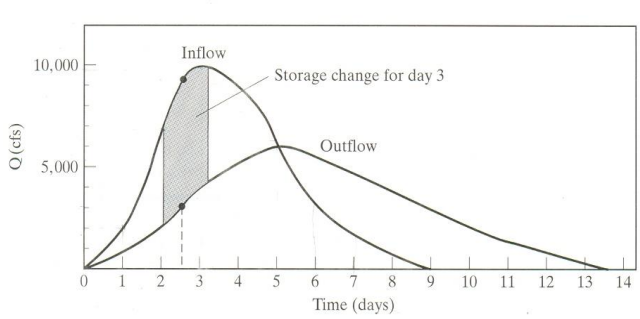
\includegraphics[width=0.5\textwidth]{hs11.png}
  \caption{Almacenamiento en un cauce al pasar una avenida}
  \label{hs11}
\end{figure}

% Clasificación de flujos en canales

% \begin{minipage}[t][3.5cm]{\textwidth}
%     \begin{center}
%     \smartdiagramset{
%     uniform color list=gray!60!black for 3 items,
%     back arrow disabled=true,
%     additions={
%     additional item offset=0.85cm,
%     additional item border color=red,
%     additional arrow color=red,
%     additional arrow tip=stealth,
%     additional arrow line width=1pt,
%     additional arrow style=]-latex’,
%     }
%     }
%     \smartdiagramadd[flow diagram:horizontal]{%
%     PGF,Ti\textit{k}Z,Smartdiagram%
%     }{%
%     below of module1/Low Level, below of module3/High level%
%     }
%     \smartdiagramconnect{{]-latex’}}{additional-module1/module1}
%     \smartdiagramconnect{{latex’-[}}{additional-module2/module3}
%     \end{center}
%     \end{minipage}
\begin{figure}[h!]
\centering
  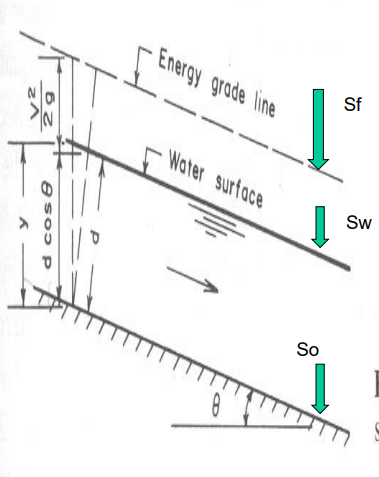
\includegraphics[width=0.5\textwidth]{hs12.png}
  \caption{boceto de definición para canal con pendiente}
  \label{hs12}
\end{figure}
Ecuaciones de Saint Venant (continuidad y momentum) Flujo no permanente unidimensional
\begin{align}
    \frac{\partial ay}{\partial t} + D \frac{\partial iV}{\partial x} + V \frac{\partial y}{\partial x} = 0\\
    \frac{\partial V}{\partial t} + V \frac{\partial V}{\partial x} + g \frac{\partial y}{\partial x} = g\left(S_0 - S_f\right)
\end{align}
Ecuación Momentum o ecuación Dinámica
\begin{equation}
    S_f = S_0 -\frac{\partial\left(\frac{V^2}{2g} + y\right)}{\partial x} - \frac{1}{g}\frac{\partial v}{\partial t} 
\end{equation}
Ecuaciones completas de saint-venant para tránsito de avenidas en cauces (Ecuaciones diferenciales parciales hiperbólicas que se resuelven con métodos numéricos) 

conservación de masa:
\begin{equation}
    y \frac{\partial v}{\partial x} + v \frac{\partial y}{\partial x} + \frac{\partial y}{\partial t} = \frac{q}{B}
    \label{eqhs2}
\end{equation}
Conservación de cantidad de movimiento:
\begin{equation}
    \frac{\partial v}{\partial t} + v\frac{\partial V}{\partial x} + g \frac{\partial y}{\partial x} = g\left(S_0 - S_f\right)
    \label{eqhs3}
\end{equation}
Los métodos hidrológicos utilizan simplificaciones de las ecuaciones \eqref{eqhs2} y \eqref{eqhs3} para llegar a soluciones más simples, pero menos aproximadas que las que se logran con los métodos hidráulicos. 
% TODO: FIx
% En este apartado se estudiará uno de éstos métodos llamado método de \textbf{Muskingum} \footnote{Tránsito de Avenidas en cauce bajo el método de Muskingum supone flujo uniforme propiedad que es utilizada para encontrar los parámetros K y x del método de Muskingum}.
\subsubsection{Método de tránsito de avenidas en cauces con el método hidrológico de muskinghum}
Éste método fue presentado en 1938, utiliza la ecuación de continuidad en su forma discreta:
\begin{equation}
    \frac{I_i + I -{i 1}}{2}\cdot \Delta t -\frac{O_i + O_{i +1}}{2}\cdot\Delta t =\Delta V
\end{equation}
y una relación algebráica entre el almacenamiento en el tramo $V$ y las entradas $I$, y salidas $O$ de la forma:
\begin{equation}
    V = K\cdot O + Kx(I - O) = K\left[ xI +(I - x)O\right]
\end{equation}
donde $K$ es una constante llamada parámetro de almacenamiento y $x$ es un factor de peso que expresa la influencia relativa de las entradas y las salidas del almacenamiento en el tramo.
Software para el Transito de Avenidas (TAV):
\begin{itemize}
    \item Presas: Método semigráfico \begin{itemize}
        \item Hms
        \item Tau IMTA, Tau CONAGUA, TAV software Ay
    \end{itemize}
    \item Cauces: Método de Muskingum \begin{itemize}
        \item HEC-HMS
    \end{itemize}
\end{itemize}

\begin{align}
    &V_{i+1}=V_i+\text{Aportaciones}_i +Vprec_i -Vevap_i-\text{Demandas}_i\\
    &V_{prec} = L_{\text{prec mediana}} (A_i+ A_{i+ 1})2\\
    &V_{evap}= L_{\text{evap mediana}}(A_i+A_{i+1})2
\end{align}
Las entradas, a veces se les llama Aportaciones Deducidas porque se deducen después que terminó el mes, reacomodando la ecuación de balance en el vaso de almacenamiento. Por lo que aportaciones deducidas para el río son igual a:
\begin{equation}
    \text{Entradas}_i=V_{i+1}-V_i -Vprec_i +Vevap_i+\text{Demandas}_i
\end{equation}
Frecuentemente no se mide la infiltración, por lo que cuando las entradas deducidas salen negativas, significa que no hubo entradas como tal, pero sí hubo infiltración.
Y los volúmenes en el vaso de almacenamiento, deben oscilar entre volumen mínimo (capacidad muerta quizá) y un volumen máximo (NAMO) de lo contrario habrá déficits o derrames.
\begin{align}
    &V_{i + 1}= V_i+ \text{Entradas}_i +Vprec_i -Vevap_i -\text{Demandas}_i\\
    &V_{\min }\leq V_i\leq V_{\max}\\
    &Si\, V_i<V_{\min },\, \text{entonces hay un deficit } =V_{min}- V_i\, \text{ y },\, V_i\quad  \text{terminará siendo } V_{min}\\
    &Si\, V_i> V_{\max },\,\text{entonces hay un derrame } = V_i- V_{max},\, \text{ y },\, V_i\quad \text{terminará siendo } V_{max}
\end{align}
\begin{table}[h!]
    \centering
    \begin{tabular}{@{}cc@{}}
    \toprule
    NORMA                                                         & LIMITE  \\ \midrule
    Deficiencia máxima anual                                      & 60\%  \\
    Deficiencia máxima para dos años consecutivos, sumados        & 90\%  \\
    Deficiencia máxima para tres años consecutivos, sumados       & 110\%  \\
    Deficiencia media anual máxima permisible                     & 5\% \\
    Deficiencia máxima para dos años consecutivos, el más seco    & 55\%   \\
    Deficiencia máxima para tres años consecutivos, el más   seco & 50\%   \\
    Máximo número de años con deficiencia en el periodo & 25 \% (si el periodo es 20 años, entonces son 5 años) \\
    Máximo número consecutivos de años con deficiencia            & 3 años  \\
    Deficiencia máxima mensual                                    & 100\%  \\ \bottomrule
    \end{tabular}
    \caption{NORMA DE DEFICIT QUE UTILIZA LA CONAGUA PARA CONSIDERAR COMO SUMINISTRO SEGURO EL DE UNA PRESA DE ALMACENAMIENTO EN BASE A UN FUNCIONAMIENTO DE VASO MENSUAL PARA PERIODOS LARGOS (CON 20 AÑOS MINIMO)}
    \label{tabhs12}
\end{table}
\subsection{Estimación del volumen útil de un vaso de almacenamiento}
\begin{figure}[h!]
\centering
  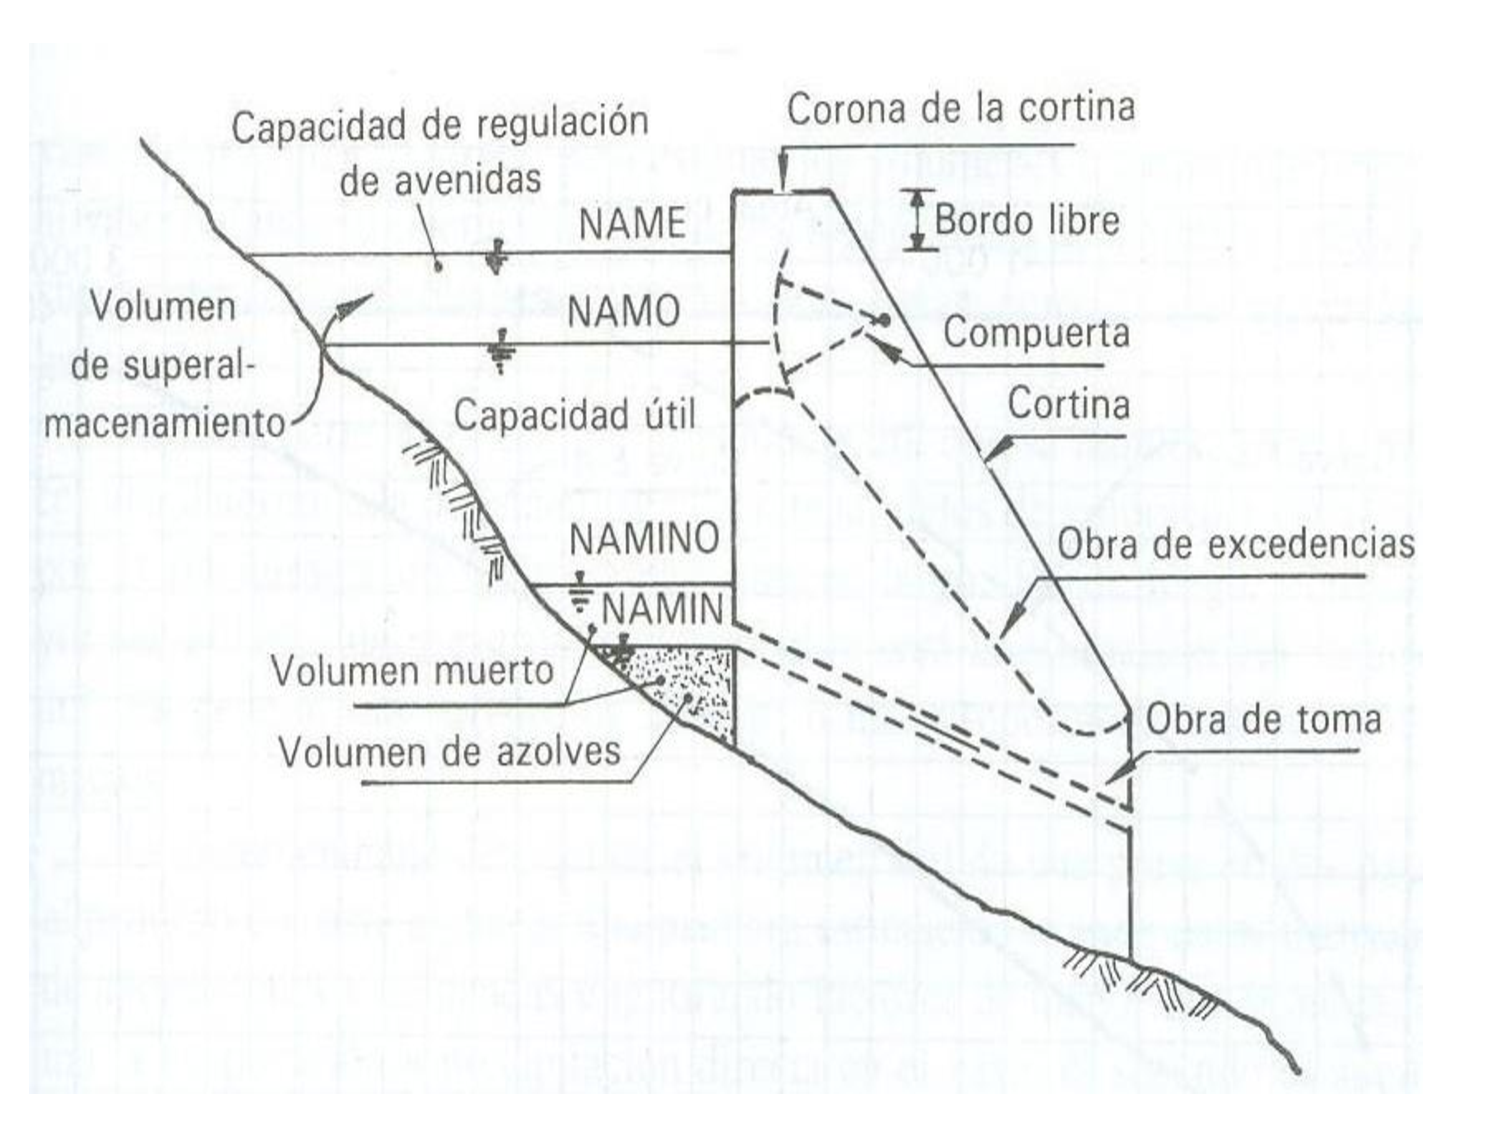
\includegraphics[width=0.5\textwidth]{hs13.pdf}
  \caption{Capas de una presa}
  \label{hs13}
\end{figure}
\begin{figure}[h!]
    \centering
      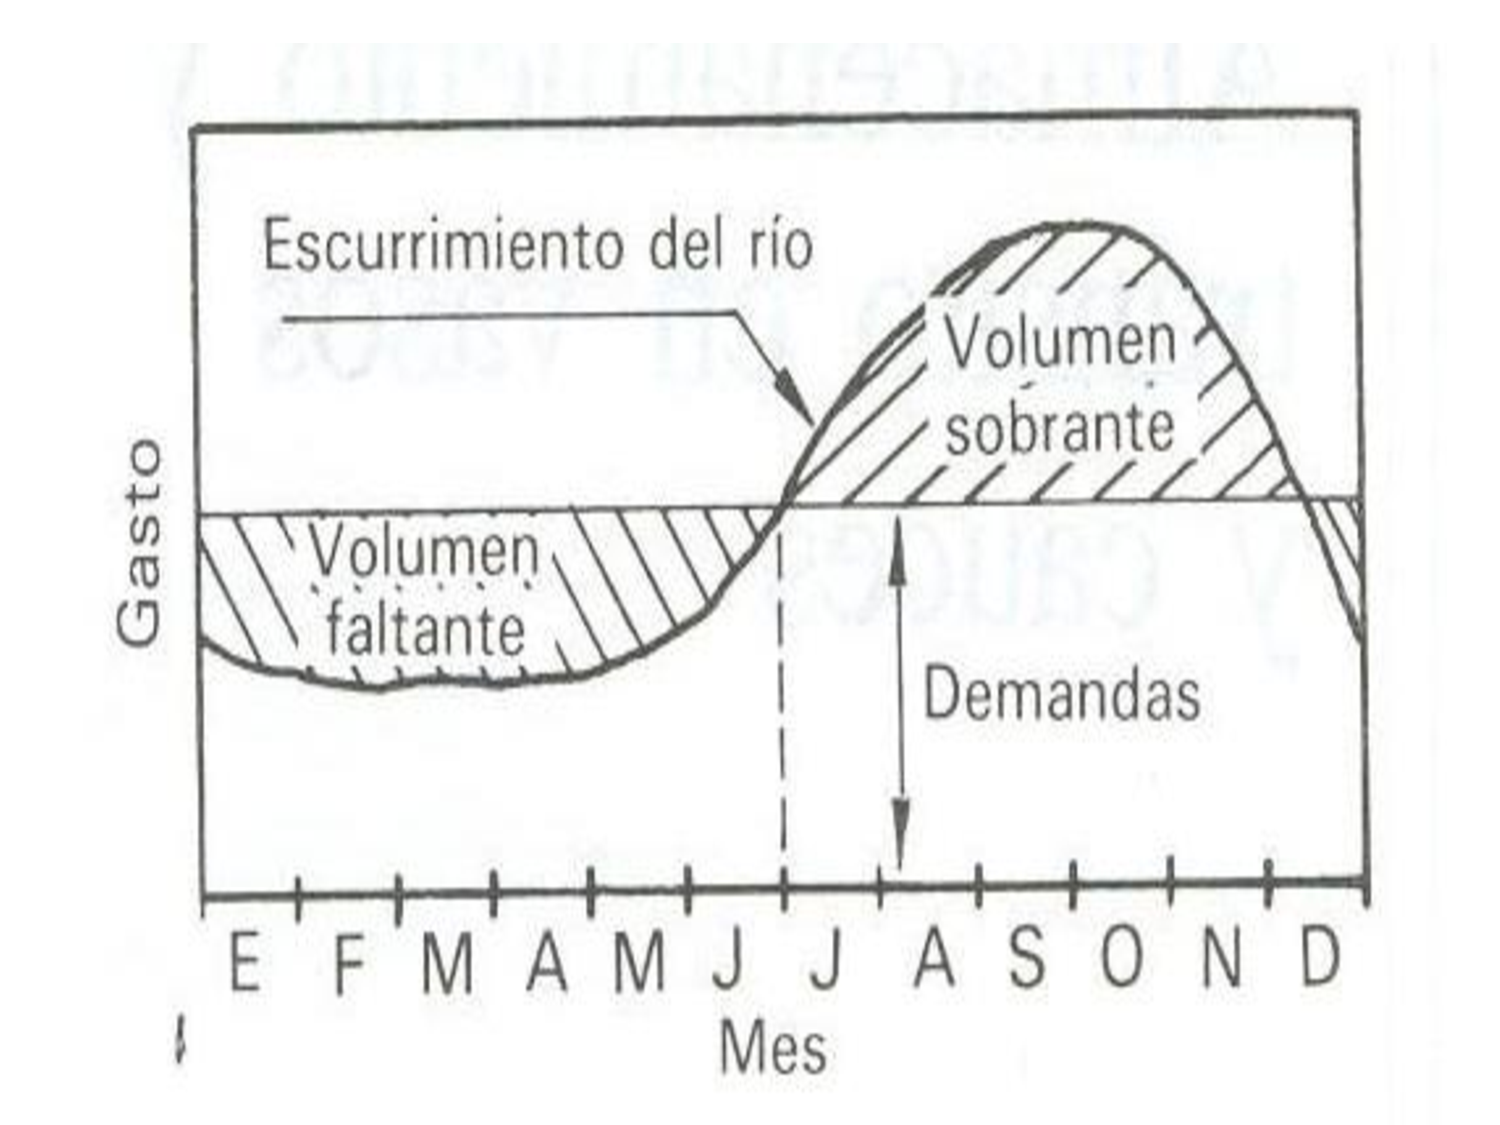
\includegraphics[width=0.5\textwidth]{hs14.pdf}
      \caption{Capas de una presa}
      \label{hs14}
\end{figure}
\begin{itemize}
    \item Método de la Curva masa o diagrama de Rippl para demandas constantes
    \item Método del algoritmo de los picos secuentes para demandas variables
\end{itemize}
Ambos métodos pueden ser completados con un estudio de funcionamiento de vaso que al detalle considera todas las entradas y salidas.

Se necesita saber los volúmenes escurridos mensuales y las demandas.

Para estimar el volumen útil de una presa que se requiere para satisfacer una determinada demanda, se deben tener registros de volúmenes escurridos por el río durante un tiempo relativamente largo (mínimo 20 años)

En ambos métodos los cálculos utilizan datos mensuales de escurrimientos y demandas e ignorando factores de menor importancia (Evaporación y Precipitación directa en el vaso)

En una segunda ``afinada'' de ambos métodos se simula el funcionamiento para todo el periodo, considerando variaciones mensuales y anuales de aportaciones y demandas y ahora si se consideran a las precipitaciones y evaporaciones directas del vaso de almacenamiento, lo cual a su vez requiere las curvas elevacionesáreas-capacidades de la presa de almacenamiento

\subsubsection{Método de la Curva masa o diagrama de Rippl para demandas constante}
\begin{figure}[h!]
\centering
  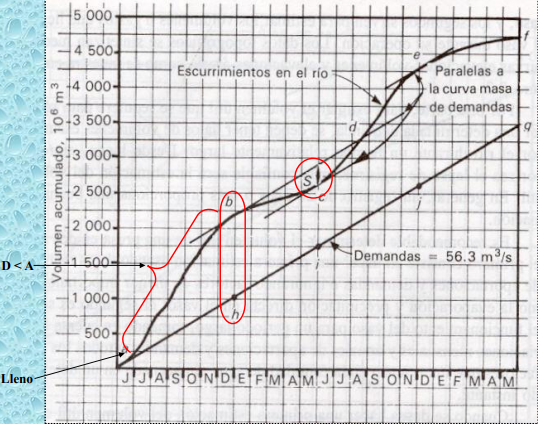
\includegraphics[width=0.5\textwidth]{hs15.png}
  \caption{Gráfica de Curva-masa de volúmenes y Demanda constante}
  \label{}
\end{figure}\begin{enumerate}
    \item Entre a y b la demanda < aportación, el vaso permanece lleno y el exceso sale por la obra de excedencias.
    \item Hasta el punto b, se ha derramado un volumen igual a la diferencia de ordenadas entre los puntos b y h, que, en el caso de la figura, es de aproximadamente $1 175 \times  106 m^3$
    \item Del punto b al c el gasto de aportación < de demanda, por lo que en este lapso, el volumen almacenado, y por lo tanto también el nivel del agua en el vaso, disminuye.
    \item En el punto c se llega a un nivel mínimo en el vaso; la máxima diferencia entre el volumen de aportación y el de demanda del punto b al c está dado por la diferencia de ordenadas S entre una recta tangente al punto b y el punto c.
    \item Del punto c al e el gasto de aportación es nuevamente mayor que el de demanda y el volumen almacenado aumenta otra vez.
    \item Para que durante el lapso indicado no se tenga déficit, el volumen útil mínimo necesario es S. El punto c corresponde al NAMINO.
\end{enumerate}
La línea $abde$ es una curva masa de salidas totales de la presa (demanda + derrames) que tiene una pendiente mínima de $56.3 m^3/s$.
\subsubsection{Método del Algoritmo del pico secuente}
\begin{enumerate}
    \item Calcular la entrada neta al vaso $\left(X_i-D_i\right)$ y la entrada neta acumulada $\sum \left(X_i-D_i\right)$
    \item Encontrar el primer pico (valor máximo) de las entradas netas acumuladas (P1 equivale a la diferencia de ordenadas b y h)
    \item Localizar el pico secuente, el siguiente pico mayor que $P_1$, equivale a la diferencia de e y j.
    \item Entre el primer par de picos, hallar el valor más bajo. Este corresponde a la diferencia de los puntos c e i y la diferencia $T_1-P_1$ equivale al volumen S.
    \item Buscar los siguientes picos secuentes y valores mínimos.
\end{enumerate}
La capacidad mínima útil necesaria para que no se tenga déficit en el periodo de los datos es, como el caso de la curva masa:
\begin{equation}
    S_u =\max{\left(P_j- T_j\right)}
\end{equation}
Para conocer el estado del vaso se le suma al valor de Su el valor de la entrada neta $\left(X_i - D-i\right)$ y cuando se rebasa el valor de Su, el exceso se va a la columna de Derrames.
\begin{table}[h!]
    \centering
    \begin{tabular}{@{}ccccccccc@{}}
    \toprule
    MES & Xi           & Di       & Xi - Di   & (Xi - Di) &    & Volúmen & Derrame & Estado   \\ \midrule
        & Aportaciones & Demandas & Acumulado &           &    &         &         & del vaso \\
        & \multicolumn{7}{c}{Miles de metros cúbicos}                              &          \\
    1   & 120          & 220      & -100      & -100      &    & 920     &         &          \\
    2   & 130          & 250      & -120      & -220      &    & 800     &         &          \\
    3   & 115          & 305      & -190      & -410      &    & 610     &         &          \\
    4   & 125          & 480      & -355      & -765      &    & 255     &         &          \\
    5   & 140          & 305      & -165      & -930      &    & 90      &         &          \\
    6   & 325          & 250      & 75        & -855      &    & 165     &         &          \\
    7   & 450          & 220      & 230       & -625      &    & 395     &         &          \\
    8   & 590          & 180      & 410       & -215      &    & 805     &         &          \\
    9   & 380          & 150      & 230       & 15        &    & 1020    & 15      & Lleno    \\
    10  & 280          & 150      & 130       & 145       &    & 1020    & 130     & Lleno    \\
    11  & 190          & 160      & 30        & 175       & P1 & 1020    & 30      & Lleno    \\
    12  & 110          & 200      & -90       & 85        &    & 930     &         &          \\
    1   & 120          & 220      & -100      & -15       &    & 830     &         &          \\
    2   & 130          & 250      & -120      & -135      &    & 710     &         &          \\
    3   & 115          & 305      & -190      & -325      &    & 520     &         &          \\
    4   & 125          & 480      & -355      & -680      &    & 165     &         &          \\
    5   & 140          & 305      & -165      & -845      & T1 & 0       &         & Vacío    \\
    6   & 325          & 250      & 75        & -770      &    & 75      &         &          \\
    7   & 450          & 220      & 230       & -540      &    & 305     &         &          \\
    8   & 590          & 180      & 410       & -130      &    & 715     &         &          \\
    9   & 380          & 150      & 230       & 100       &    & 945     &         &          \\
    10  & 280          & 150      & 130       & 230       &    & 1020    & 55      & Lleno    \\
    11  & 190          & 160      & 30        & 260       & P2 & 1020    & 30      & Lleno    \\
    12  & 110          & 200      & -90       & 170       &    & 930     &         &          \\ \bottomrule
    \end{tabular}
    \caption{Demandas variables}
    \label{tabhs13}
    \end{table}
La capacidad mínima útil necesaria para
que no se tenga déficit en el periodo de los
datos es, como el caso de la curva masa:
\begin{align}
    S_u =\max{\left(P_j - T_l\right)}\\
    S =\left(175 -( - 845)\right) = 1020\times 10^3m^3
\end{align}
% \subsection{Sedimentos}
% La determinación del volumen util da lugar al NAMO, el tránsito de avenidas de una creciente máxima ($Q_{\max}$) daba lugar al NAME, finalmente los sedimentos anuales + la vida util de la presa da lugar al NAMIN.

% Los sedimentos cuando se originan en una ladera, se debe transitar el cauce mediante programas como SWAT para saber cuánta deposición hay.

% Se da el nombre genérico de sedimentos a las partículas procedentes de las rocas o suelos y que son acarreadas por las aguas que escurren.

% Todos estos materiales, después de cierto acarreo finalmente son depositados a lo largo de los propios cauces, en lagos, presas de almacenamiento.

% Hay erosión hídrica por deslizamiento en laderas, transporte y deposición de sedimentos en los cauces de los ríos.

% La cantidad de sedimentos producidos por la cuenca y transportados a través del cauce hasta llegar a la presa, la eficiencia de la presa para atrapar sedimentos.

% Volumen azolves en un vaso de almacenamiento $m^3$
% \begin{equation}
%     Vaz = \frac{N}{W_y}
% \end{equation}

% \subsubsection*{Eficiencia de atrapado de sedimentos en la presa}
% La eficiencia es la proporción del sedimento que viene en los escurrimientos y que es atrapado en el embalse
% \begin{equation}
%     E_a = 100\cdot\left(\frac{}{}\right)
% \end{equation}
% EL volumen de sedimentos en $m^3$
% \begin{equation}
%     a
% \end{equation}
% el ultimo destino de todos los sedimentos son los fondos de los embalses. Grandes producciones de sedimentos acortan la vida útil de un embalse.

% Para determinar la capacidad muerta de un embalse (para azolves) se debe considerar la producción de sedimentos para los N años 

% \begin{equation}
%     W_t =\frac{\%Arena}{100}
% \end{equation}
% Tiempo que lleva azolvar ese volumen a perder
% \begin{equation}
%     T_s = \frac{V}{V_s \cdot E}
% \end{equation}
% La sedimentación no puede ser prevenida pero si retardada. Una forma de hacer esto es seleccionar un sitio donde el flujo de sedimentos sea bajo.

% Los métodos de conservación de suelo (terrazas, cultivos en contorno), proteger margenes de































































